\documentclass[a4paper,12pt]{article}

% for code presentation
\usepackage{listings} 
\usepackage{color}
\usepackage{longtable}
\usepackage{hyperref}
\setcounter{secnumdepth}{5}
\definecolor{dkgreen}{rgb}{0,0.6,0}
\definecolor{gray}{rgb}{0.5,0.5,0.5}
\definecolor{mauve}{rgb}{0.58,0,0.82}
\lstset{frame=tb,
  language=Java,
  aboveskip=3mm,
  belowskip=3mm,
  showstringspaces=false,
  columns=flexible,
  basicstyle={\small\ttfamily},
  numbers=none,
  numberstyle=\tiny\color{gray},
  keywordstyle=\color{blue},
  commentstyle=\color{dkgreen},
  stringstyle=\color{mauve},
  breaklines=true,
  breakatwhitespace=true,
  tabsize=3
}

\usepackage{graphicx} % for image inclusion
\graphicspath{{./images/}}

\begin{document}
\title{\textit{GPL} \\ Final Report}
\author{Qingxiang Jia (qj2125)\\ Peiqian Li (pl2521)\\ Ephraim Donghyun Park (edp2114)}
\maketitle
\tableofcontents
\newpage

\section{Introduction}
GPL (Graph Programming Language) is designed for graph related programming. It has intuitive ways of declaring graphs as well as the built-in data types for graph and its components such as edges and nodes. Its syntax is similar to C-like main stream imperative languages. It also supports user defined functions. With GPL, the user can easily built graphs and graph-related algorithms to solve real life problems. GPL is compied into C, which can then be compiled into machine code using gcc or clang.

\subsection{Motivation}
While graph is an important part in Computer Science and Mathematics, there are not many programming languages with built-in support for graph, not mentioning an intuitive way of describing the data structure of a graph. We decided to build GPL to discover the possibilities.

\subsection{Key Features}
\begin{description}
	\item[Intuitive Graph Declaration] \hfill \\ 
	One can declare an undirected or directed graph by using a combination of dashes and greater-than symbol. One can express the weight of an edge by including a number, or a string or even an expression in the parenthesis. One can also refer to the weight by dot operator. This will be explained in detail in the next section.
	\item[User Defined Function] \hfill \\
	The user can defined their own functions. This expands the expressiveness of GPL, and make it more flexible. With the support of user defined function, GPL can easily express simple algorithms such as GCD in recursive or iterative fashion; more complicated algorithm such as Kruskal's minimum spanning tree algorithm can also be expressed.
	\item[Complete Control Structures] \hfill \\
	GPL has most of the popular structures appeared in main stream programming languages such as for and while loops, if and if else statements. More details will be revealed in the next section. 
\end{description}

\section{Language Tutorial}
\subsection{Basic Structure of A GPL Program}
Unlike many popular programming languages, GPL is not object-oriented, therefore, it does not support class, or struct. A basic program consist of a main function. As simple as it sounds, this all it needs. For example, the simplest GPL program and a hello-word example are provided below.
\begin{lstlisting}
// the simplest GPL program
void main() {
}
// hello word
void main() {
	print("Hello World!");
}
\end{lstlisting}

\subsection{Built-in Data Types and Variable Assignment}
GPL supports a set of primitive types, integer (int), character (char) and string (string). Notice that in GPL, string is also a primitive type. The following code illustrates the how to assign values for built-in data types.
\begin{lstlisting}
int main() {
	int i = 41;
	char c = '4';
	string s = "43";
	// you can also declare first and assign later
	char k;
	k = 'k';
	return 0;
}
\end{lstlisting}

\subsection{Control Structures}
The following code illustrates the usage of for loop, while loop, and if statements. In short, the syntax is similar to C's.
\begin{lstlisting}
void main() {
	int soln = 42;
	if (soln == 42) { // the { } can be omitted here
		print("That is the answer.\n");
	}
	int num = 0;
	for (int i = 0; i < 10; i+=1)
		num += 1; // ++ or -- is not support; +=, -=, /=, *=, %= are
	while (num > 0)
		num -= 1; // can also use num += -1;
	if (num == 0 && soln == 42) // or operator is ||
		print("Running correctly.\n");
}
\end{lstlisting}

\subsection{Writing and Calling a Function}
The first part of the function is return type, if none, use ``void". However, as the entry point of any GPL program, main() has to be void. The second part is function body, surrounded by curly brackets. Below is an example of a recursive GCD algorithm that illustrates the usage of function.
\begin{lstlisting}
int gcd(int a, int b) {
	if (b == 0)
		return a;
	else
		return gcd(b, a % b);
}

void main() {
	print(gcd(20, 40));
}
\end{lstlisting}

\subsection{Advanced Date Types}
For all primitive types, GPL has a corresponding array type. Different from the main stream programming style, to declare an array, the size of the array is explicitly written in ``[ ]" on the left side. The following example illustrate that.
\begin{lstlisting}
void main() {
	int[3] a; // initialized to 0
	a[2] = 2;
	print(a[2]); // should print 2
}
\end{lstlisting}

\subsection{Defining a Graph}
The following three ways of defining the simple graph shown below are equivalent. They all result in the same representation as the following figure.
\begin{figure}[h]
	\centering
	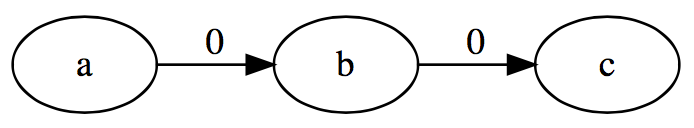
\includegraphics[scale=0.5]{a->b->c.png}
\end{figure}
\begin{lstlisting}
void main() {
	graph g1 = [
		a -> b -> c;
	];
	graph g2 = [
		a -> b;
		b -> c;
	];
	graph g3 = [
		b -> c;
		a -> b;
	];
}
\end{lstlisting}

\subsubsection{Defining a Graph with Redundancy}
The syntax is the exactly the same. The purpose of the illustration is to show that GPL will sort out the graph even though some lines in the definition could be redundant. The bottom line is that there should be no conflict in the definitions of a graph. In this illustration, we define a loop. GPL will ignore the redundant part in definitions.
\begin{figure}[h]
	\centering
	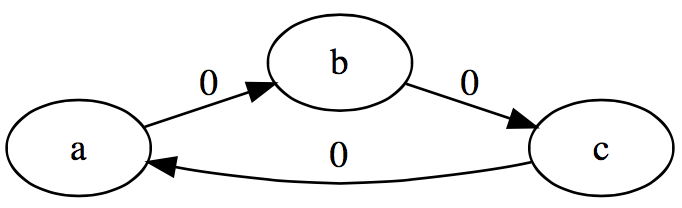
\includegraphics[scale=0.5]{a->b->c->a.png}
\end{figure}
\begin{lstlisting}
void main() {
	graph g1 = [
		a -> b -> c -> a;
		a -> b; // ignored
		c -> a; // ignored
		b -> c; // ignored
	];
}
\end{lstlisting}

\subsubsection{Defining a Graph with Edge Weights}
This is probably the most creative and intuitive way of defining a graph with edge weights. Weights are flexible in terms of the form, it can be of as simple as an int type, or an expression that results in an value of type int. Notice that defining a weight for an edge is optional in graph. The default weight is zero. The following illustrates how to define a graph equivalent to the figure shown below.
\begin{lstlisting}
void main() {
	graph g1 = [
		a -(1)> b -(2)> c -> a;
	];
}
\end{lstlisting}

\begin{figure}[h]
	\centering
	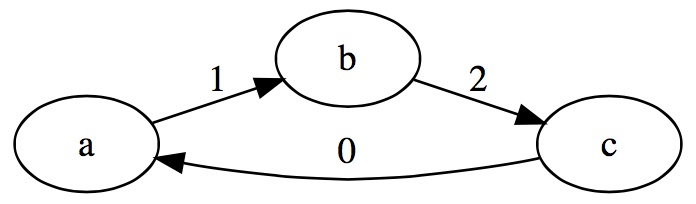
\includegraphics[scale=0.5]{a-(1)>b-(2)>c->a.png}
\end{figure}

As mentioned previously, expressions that are evaluated as integer values can also be used as edge weights. The following example demonstrates it.
\begin{lstlisting}
void main() {
	int l = 2;
	int m = 2%a;
	graph g1 = [
		a -(l)> b -(l*m+2)> c -(m)> a;
	];
}
\end{lstlisting}
Below is the image representation of the graph defined above.
\begin{figure}[h]
	\centering
	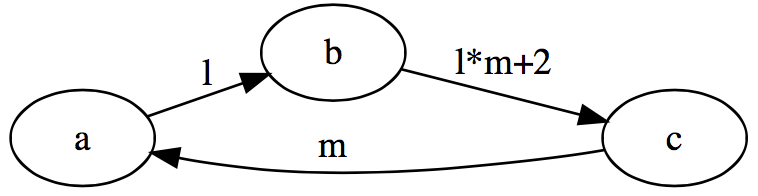
\includegraphics[scale=0.5]{expr_as_weight.png}
\end{figure}

\section{Language Manual}
\subsection{Introduction}
Graph is a very powerful data structure that can be used to model a variety of systems in many fields.  Graph is such a fundamental model that people have developed libraries dedicated to graphs in almost all general-purpose high-level programming languages.  However, implementing graph-related algorithms in languages like Java or C++, even with the benefit of using third-party graph libraries, entails manual manipulation of nodes and edges.  This could prove to be error-prone (with pointer manipulations in C++), tedious (verbose especially in Java), and daunting (to people new to the programming world).

The Graph Programming Language (GPL) is a domain-specific language that attempts to remedy these problems.  GPL strives to hide most logic behind graph handling under the hood, so that programmers are able to focus more on using graphs, instead of implementing them.

The primary goal of GPL is to allow programmers to create, use, and manipulate graphs in a natural, flexible and intuitive way. All graph-based algorithms should be easier to implement in GPL, e.g. shortest path, spanning tree, strong connectivity. Because all trees are graphs, GPL is automatically suitable for applications involving tree structures, such as priority queues (min/max heaps), binary search trees, or any kind of hierarchical data representation.

\subsection{Lexical Conventions}
\subsubsection{Comments}
Two slashes "//" introduce one-line comment, which is terminated by the newline character. For multiline comment, /* is used to start commenting and */ is used to terminate commenting. Nested commenting is not supported by the language.

\subsubsection{Identifiers}
An identifier consists of a sequence of letters, digits, and the underscore character; the first character of an identifier cannot be a digit. Upper and lower case letters are considered different.

\subsubsection{Keywords}
The following identifiers are reserved by the language to have specific meanings and may not be used otherwise:

\begin{tabular}{ l l l }
\hline
boolean & break & char \\
continue & edge & else \\
for & graph & if \\
int & node & return \\
string & while \\
\hline
\end{tabular}

\subsubsection{Object Type}
In GPL, graph, edge, node, and string are object types. "Object" implies that they are not primitive data types, and they can have member functions and fields which can be invoked or accessed through the dot operator. Graph, node, edge, and string are the only four object types in GPL; GPL does not support user-defined objects, but does support user-defined functions.

\subsubsection{Literals}\paragraph{Integer literals}
Integer literals are decimal (base 10). An integer literal is just a sequence of digits.
\paragraph{Character literals}
A character literal is one or two characters enclosed by single quotes. Two characters enclosed by single quotes are for escape characters. The first character must be back-slash, and the second one can be back-slash, single quote, 'n', 'r', 't'; they represent backslash, single-quote, line-feed, carriage-return, and tab, respectively. The only valid representation of the single-quote character is a back-slash followed by a single-quote, enclosed in two single quotes.

\paragraph{Boolean literals}
There are exactly two boolean literals: \textbf{true} and \textbf{false}.

\paragraph{String literals}
A string literal is a sequence of characters enclosed by double quotes. Backslash, double-quote, line-feed, carriage-return, and tab characters need to be escaped by a preceding back-slash, similar to character literals.

\paragraph{Graph literals}
A graph literal is a list of weighted directed edges enclosed by square brackets. All weights must be integers. Only directed edges are supported by GPL.

\subsection{Expressions}
\subsubsection{Primary Expressions}
\paragraph{identifier}
An identifier is a unique (in its own scope) name used to identify an entity in the program. It can be the name of a function, parameter, or variable.  A reserved keyword cannot be used as an identifier.

For array identifier, the following member functions can be used:
\begin{center}
\begin{tabular}{| l | p{10cm} |}
\hline
	len()		& this member function returns the size of the array \\ \hline
	sort()  & this member function can only be used for int, char, or edge arrays and it sorts the element \\ \hline
\end{tabular}
\end{center}


\paragraph{literal}
Literals include strings, characters, numbers (integer), and graphs.

\paragraph{string}
String is an object type of the language. String is immutable.

String has the following two member functions:
\begin{center}
\begin{tabular}{| l | p{10cm} |}
\hline
	len()		& this member function returns the length of the string \\ \hline
	substr(a, len)  & this member function returns the substring starting at index \textbf{a}, and includes \textbf{len} characters. \\ \hline
	empty()	& this member function returns true if the string is empty \\ \hline
	at(i)		& this member function returns the character at the specified index \\ \hline
	append(s)  & this member function appends s to the called string \\ \hline
\end{tabular}
\end{center}

\paragraph{node}

	Node is an object type of the language. It represents a node in a graph.
	
	Node has member function:
\begin{center}
\begin{tabular}{| l | p{10cm} |}
\hline
getID()	&	returns the unique integer ID of the specified node \\ \hline
\end{tabular}
\end{center}

\paragraph{edge}

	Edge is an object type of the language. It connects two nodes.
	
	Edge has member functions:
\begin{center}
\begin{tabular}{| l | p{10cm} |}
\hline
		getWeight()	&	returns the weight of the edge. \\ \hline
		getSrc()  	&      returns the source node of this edge. \\ \hline
		getDst()	&	returns the destination node of this edge. \\ \hline
		
\end{tabular}
\end{center}
		
\paragraph{graph}
Graph is an object type of the language. It represents a directed graph which consists of nodes and directed edges with integer weights. 

The nodes in a graph can be accessed like fields. For example, if graph g has node v, then the node is represented by the expression "g.v".

Graph has member functions:
\begin{center}
\begin{tabular}{| l | p{10cm} |}
\hline
	getNode(int id)	&	returns the node with specified id \\ \hline
	getEdge(node src, node dst)	&	returns the specified edge. If the specified edge does not exist, a run-time exception is raised.\\ \hline
	getAllEdges()	&	returns the list of edges in the graph as an array\\ \hline
	getAllNodes()	&	returns the list of nodes in the graph as an array\\ \hline
	getWeight(node src, node dst) 	&	returns the weight of the edge that goes from src to dst node \\ \hline
	getEdgeCount() 	&  returns the number of edges in the graph \\ \hline
	getNodeCount()	&  returns the number of nodes in the graph \\  \hline
	getInNeighbours(node n)	&	returns an array of nodes that have edge to the specified node \\ \hline
	getOutNeighbours(node n) &	returns an array of nodes that this node has edges to \\ \hline

	
\end{tabular}
\end{center}

\paragraph{( expression )}
The parenthesized expression is the same as expression. Including an expression in a pair of parentheses does not imply any precedence of the expression.

\paragraph{primary-expression {[} expression {]} }
The primary-expression in this part can only be array. The expression can only be integers within the range of the array. primary-expression [ expression ] means to access the expression-th element in the array.

\paragraph{primary-expression ( expression ) }
This expression means a functional call, where primary-expression is an identifier that is a name of a function. The expression in the pair of brackets is parameter(s) to in the call. It can be single parameter. If there are more than one parameters, they should be separated by a comma.

\paragraph{primary-lvalue . member-function-of-object-type}
An lvalue expression followed by a dot followed by the name of a member function of object-type is a primary expression.

\subsubsection{Graph Definition Operators}
%\subsubsection{expression $--$ expression}
%The $--$ binary operator connects two nodes with unweighted undirected edge.

\paragraph{identifier $->$ identifier}
The $->$ binary operator connects two nodes with zero-weighted directed edge. The direction goes from first node identifier to second node identifier.

%\subsubsection{expression $--$: expression, expression, ...}
%The $--$: operator connects first node expression with all the other node expressions that follow with unweighted undirected %edge.

\paragraph{identifier :$->$ identifier, identifier, ...}
The :$->$ operator connects first node identifier with all the other node identifier that follow with zero-weighted directed edge.

%\subsubsection{expression $-$(expression)$-$ expression}
%The $-$(expression)$-$ operator connects two nodes with weighted undirected edge. The weight of the edge equals the %expression in the middle.

\paragraph{identifier $-$(expression)$>$ identifier}
The $-$(identifier)$>$ operator connects two nodes with weighted directed edge. The direction goes from first node identifier to second node identifier. The weight of the edge equals the expression in the middle. The expression must be of int type.

%\subsubsection{expression $-$(expression)$-:$ expression, expression, ... }
%The $-$(expression)$-:$ operator connects first node expression with all the other node expressions what follow with %weighted undirected edge. The weight of the edge equals the expression in the middle.

\paragraph{identifier $:-$(expression)$>$ identifier, identifier, ... }
The $:-$(expression)$>$ operator connects first node identifier with all the other node identifier what follow with weighted directed edge. The weight of the edge equals the expression in parentheses. The expression must be of int type.

\subsubsection{Unary Operators}
Unary operators are grouped from right to left.
\paragraph{$-$ expression}
The $-$ unary operator can be applied to an expression of type int or char, and results in the negative of the expression.

\paragraph{$!$ expression}
The $!$ unary operator can only be applied to an expression of boolean type, and results in the opposite of the truth value of the expression

\subsubsection{Multiplicative Operators}
\paragraph{expression * expression}
The binary operator * indicates multiplication between expression and expression. The expression pair can be in the following combinations. 1) int int 2) char char 3) int char 4) char int. In case 3, and 4, all the parameters will be treated as int.
\paragraph{expression / expression}
The binary operator / indicates division between expression and expression. The expression pair can be in the following combinations. 1) int int 2) char char 3) int char 4) char int. In case 3, and 4, all the parameters will be treated as int.
\paragraph{expression \% expression}
The binary \% operator outputs the remainder from the division of the first expression by the second. The expression pair can be in the following combinations. 1) int int 2) char char 3) int char 4) char int. In case 3, and 4, all the parameters will be treated as int.
\subsubsection{Additive operators}
\paragraph{expression + expression}
The binary + operator outputs the addition of the first expression and the second expression. The expression pair can be in the following combinations. 1) int int 2) char char 3) int char 4) char int. In case 3, and 4, all the parameters will be treated as int.
\paragraph{expression - expression}
The binary - operator outputs the result of the first expression minus that of the second expression. The expression pair can be in the following combinations. 1) int int 2) char char 3) int char 4) char int. In case 3, and 4, all the parameters will be treated as int.
\subsubsection{Relational operators}
\paragraph{expression $<$ expression}
\paragraph{expression $>$ expression}
\paragraph{expression $<=$ expression}
\paragraph{expression $>=$ expression}
\paragraph{expression $==$ expression}
\paragraph{expression $!=$ expression}
The relational operators $<$ (less than), $>$ (greater than), $<=$ (less than or equal to), $>=$ (greater than or equal to), $==$ (equal to), $!=$ (not equal to) all yield boolean \textbf{true} or \textbf{false}. The two expressions being compared must be of the same type, and they can be int, float, char or string. Characters are compared by ASCII values; strings are compared lexicographically.
\subsubsection{Assignment operators}
\paragraph{variable = expression}
The binary = operator indicates that the result of the expression on the right side is stored in the variable on the left. If there is already data stored in the variable, the data will be replaced. The variable can be any legal type defined in the language.
\paragraph{variable += expression}
The binary += operator indicates that the value of the variable on the right side will be incremented by the quantity of the result of the expression on the left side. This operator requires the two expressions to be in the same numerical type, i.e. either both in int, or both in char.
\paragraph{variable -= expression}
The binary -= operator indicates that the value of the variable on the right side will be decremented by the quantity of the result of the expression on the left side. This operator requires the two expressions to be in the same numerical type, i.e. either both in int, or both in int.
\subsubsection{Logical operators}
\paragraph{boolean-expression $\&\&$ boolean-expression}
\paragraph{boolean-expression $||$ boolean-expression}
The logical operators $\&\&$ (and) and $||$ (or) can be applied to two boolean expressions, and results in the logical AND or OR of the truth values of the two boolean expressions.

\subsubsection{Function calls}
Function calls are made by function identifier followed by the list of arguments separated by commas enclosed by parentheses. Function overloading, functions with the same name but different set of argument types, is supported.

\subsection{Declarations}
\subsubsection{Type specifiers}
The type-specifiers are

\begin{lstlisting}
type-specifier:
		int
		char
		string
		graph
		node
		edge
		type-specifier [ ]
\end{lstlisting}
	
\subsubsection{Variable Declarators}
\begin{lstlisting}
declarator:
	type-specifier identifier
	type-specifier identifier = expr
\end{lstlisting}
	
\subsubsection{Graph Expression}
\begin{lstlisting}
graph-expr
	[ graph-body ]
		
graph-body
	edge-declaration-list

edge-declaration-list:
     	edge-declaration;
    	edge-declaration; edge-declaration-list 
 
edge-stmt:
     	node-declarator 
   	node-declarator -> edge-stmt 
    	node-declarator - ( expr ) > edge-stmt 
 
edge-declaration:
     	edge-stmt 
   	node-declarator : - ( expr ) > node-declarator-list  
   	node-declarator : -> node-declarator-list  
 
node-declarator-list:
     	node-declarator 
     	node-declarator node-declarator-list    
 
node-declarator:
     	identifier

\end{lstlisting}

\subsubsection{Function declarations}
\begin{lstlisting}

function-decl:
 	retval formals_opt ) { stmt_list }

  
procdecl: /*procedure (aka. void function) declarator*/
   	void identifier ( formals_opt ) { stmt_list }
  
retval:
      	vartype identifier (
 
formals_opt:
	/* nothing */ 
    	formal_list 
  
formal_list:
      	vardecl
    	formal_list , vardecl 
 
\end{lstlisting}		

\subsection{Statements}
\subsubsection{Expression statement}
Expression statement is an expression followed by semicolon.
\subsubsection{Compound statement}
The compound statement is a list of statements surrounded by parentheses.
\subsubsection{Conditional statement}
There are two types of conditional statements:

\begin{itemize}
\item Type 1: if (expression) statement
\item Type 2: if (expression) statement else statement
\end{itemize}
In type 1, if expression is evaluated to be true, the statement will be executed. In type 2, if expression is evaluated to be true, the first statement will be executed, otherwise the second statement will be executed.
\subsubsection{While statement}
The while statement can be described as: while (expression) statement

As long as the expression is evaluated to be true, the statement will be executed repeatedly. The expression is evaluated before the execution of statement.

\subsubsection{For statement}
The for statement can be expressed as: 

for (expression-1; expression-2; expression-3) statement

expression-1 defines the initialization of the loop. expression-2 is the test that will be evaluated for truth in each loop. expression-3 defines what to do after each loop has been executed.

\subsubsection{Return statement}
Return statement can be described as: return (expression)

The expression can be either a simple expression, which will be evaluated to a value and then be returned to the calling function. Alternatively, the expression can be consisted of one or more function calls, then the return statement will be executed after all function calls have been returned.

\subsubsection{Null statement}
A null statement consists a single semicolon. It is useful in a for loop where one or more of the three expressions is not defined (or unneeded to define).

\subsection{Scoping}
There are three rules of scoping. The first rule states that the global variables and functions can be referred from anywhere in the code even before it is declared. The second rule states that the variables declared in a function can be referred only after the declaration. The third rule states that the variables declared in a function bind closer than the variables declared outside the function. For example, there is a variable named a in a function, even though, outside the function, there may be a variable a, because of the stronger binding of the variable declared in the function, if one refers a in the function, he or she refers to the one declared in the function.

\section{Project Plan}
\subsection{Planning}
Our group routinely meet on Friday and Saturday, and holidays like Thanksgiving. Initially, the idea was that each of us should work on our own part individually, but as the project progressed, we realized that it is more efficient to work together in CLIC lab. We also meet with Olivia on Thursday. Since we only have three team members, scheduling a time to work together is relatively easy. Because that new problems came as we the development went further, we gave up making clear plans for each week. Instead, every time we meet, we solve a major issue encountered in that week.

\subsection{Specification}
We treated the LRM as a rough guideline of our language. At the beginning, we build the language in the format specified exactly in the reference manual, but later, we realized that the reference manual itself had many details unspecified, therefore we made the decision during the development, and came back to update the reference manual. Other problem with the early specification is that some features are too hard to implement. For example, initially, the syntax we specified in the manual on defining graph always end up in shift reduce error, and it turned with the old syntax, it cannot distinguish a block of graph content and a block of regular code. In cases like that, we modified the specification.

\subsection{Development}
We worked together in CLIC lab, using git as version control. Not only OCaml code, but also testing scripts, reports, and reference manual are hosted in GitHub. Other than the meeting with Olivia, we do not have dedicating meetings. One reason is that we only have three team members, no such meeting is necessary. The other reason is that we work together, and we have fully awareness of everyone's progress. 

\subsection{Testing}
The full automatic testing suite was written right after we finished the scanner. We have dedicated individual writing test cases for each part of the language so that the rest of the team can focus on developing. We have a large number of test cases, each case only focus on one aspect of the language. Each test case uses with the language as deviously as possible. We test both the cases where the language should fail (raising exceptions), and should not. Each test case is a pair of files. One GPL source code, one output file. The automatic test suite will compare the actual output of the source code to the expected output and decides whether it is a pass or fail.

\subsection{Programming Style Guide}
The coding style is the same as the ones presented in class. We did not enforce a specific style since we are both new to OCaml. The bottom line is that each of us can understand the code. During the process, no one has written any code that other cannot understand.

\subsection{Project Timeline}
Add a table briefly describe what we did on each day, after the project is done.
\begin{figure}[h]
	\centering
	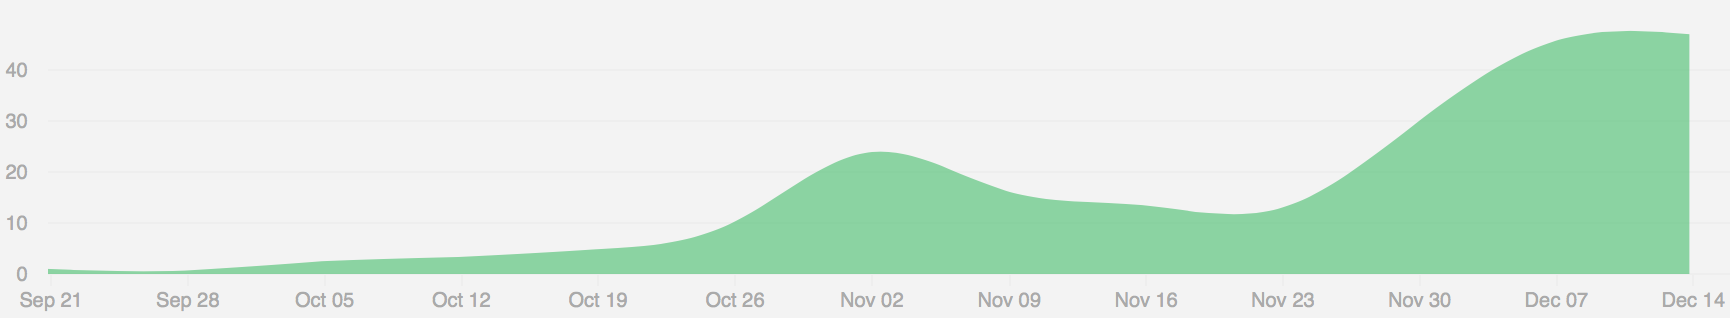
\includegraphics[scale=0.4]{git_stats.png}
	\caption{Git Statistics from Sep 21, 2014 to Dec 17, 2014}
\end{figure}
\begin{description}
  \item[Oct 10, 2014] \hfill \\
  Start writing LRM, scanner
  \item[Nov 04, 2014] \hfill \\
  Building parser, ast, testing scripts
  \item[Nov 08, 2014] \hfill \\
  Continue on parser and ast
  \item[Nov 14, 2014] \hfill \\
  Continue on parser and ast
  \item[Nov 15, 2014] \hfill \\
  AST done
  \item[Nov 21, 2014] \hfill \\
  Start writing SAST, code generation, test cases
  \item[Nov 28, 2014] \hfill \\
  Keep working on SAST, code generation, and test cases; start writing demo
  \item[Nov 30, 2014] \hfill \\
  Working on SAST, code generation, test cases, and demo
  \item[Dec 06, 2014] \hfill \\
  Updated testing scripts, building language libraries, SAST, test cases, demo
  \item[Dec 09, 2014] \hfill \\
  Working on SAST, code generation, test cases, demo, and final report
  \item[Dec 11, 2014] \hfill \\
  Same as above
  \item[Dec 14, 2014] \hfill \\
  SAST passed all test cases, building code generation, test cases, demo, and final report
  \item[Dec 15, 2014] \hfill \\
  All demos worked correctly, code generation stablized, improving SAST, final report
  \item[Dec 17, 2014] \hfill \\
  Final presentation
\end{description}

\subsection{Roles and Responsibility}
\begin{description}
	\item[Ephraim Park] \hfill \\
	The assigned role was system architect. I have worked on the scanner, parser, ast, sast, and LRM. I am the major contributor of scanner, and sast.
	\item[Peiqian Li] \hfill \\
	The assigned focus was verification and validation. I wrote the test suite, and I have worked on the scanner, parser, ast, sast, LRM, and code generation.
	\item[Qingxiang Jia] \hfill \\ 
	The assigned role was project manager and language guru. I have worked on the parser and ast, writing test cases, demo code, LRM and final report.
\end{description}

\subsubsection{Development Environment}
All of the team members work on OS X with OCaml compiler installed. The most popular editors are vim and Sublime Text. We did not use any IDE. Git is used as version control, GitHub is the host. For complicated demo, we used Python as proof of concept and then translated it into GPL.

\subsubsection{Project Log}
Attach the git log after the project is done.

\section{Architectural Design}

The architectural design of GPL is demonstrated in the following block diagram:

\begin{figure}[h]
	\centering
	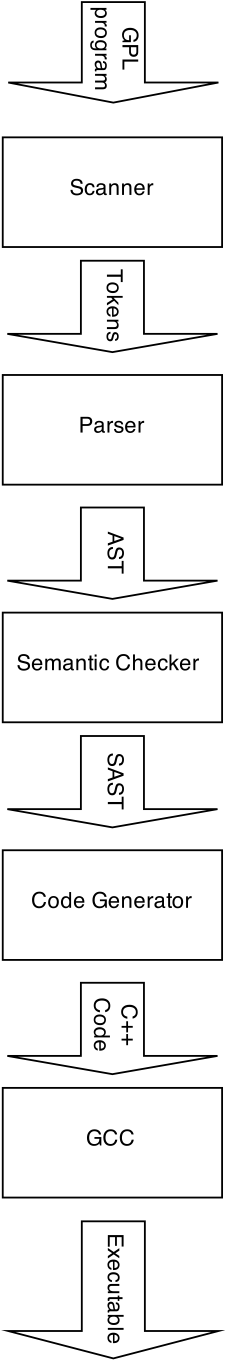
\includegraphics[scale=0.8]{block_diagram.png}
\end{figure}

Scanning and parsing were implemented by all three team members together; semantic check was done by Ephraim Park; code generation was done by Peiqian Li.

\subsection{Scanning}
We used \textbf{ocamllex} to tokenize the input source program into parsable units, to be further processed by the parser.  The scanner discards comments, tabs, newlines, and space characters.  Escaped characters or sequence of escaped characters in the source program are unescaped by the scanner before being handed to the parser.

\subsection{Parsing and Abstract Syntax Tree}
We used \textbf{ocamlyacc} to parse the scanned tokens to an abstract syntax tree, as illustrated below.  The parser rejects syntactically incorrect input programs.

\begin{figure}[h]
	\centering
	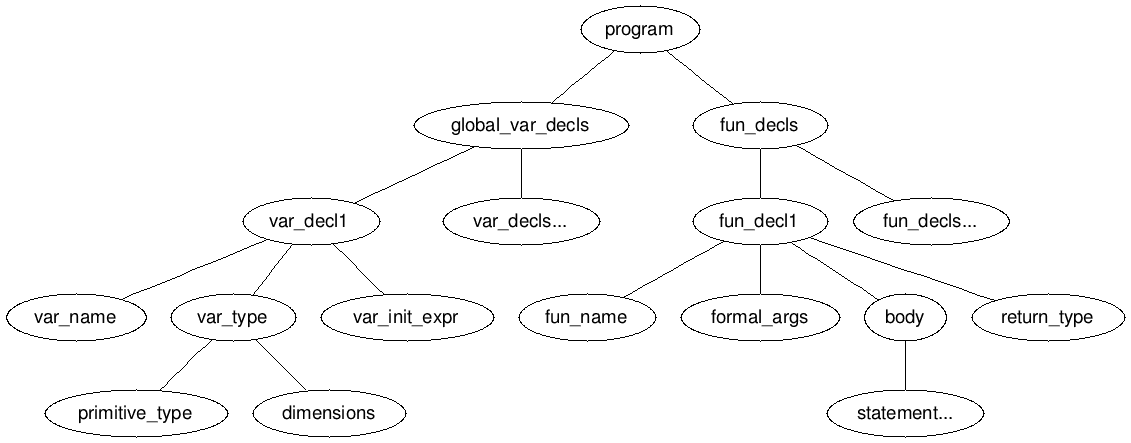
\includegraphics[scale=0.35]{ast.png}
\end{figure}

\subsection{Semantic check and SAST}
In this stage, the parsed AST is checked for various semantic errors, including reference to undefined variables or functions, type mismatch in expressions or function parameter passing, variable redefinition within the same scope.  We used a hash map to maintain variable and function references. We support function overloading by mapping a function name to a list of functions with different formal arguments.

\subsection{Code generation}
The code generator takes a semantically checked abstract syntax tree, and generates the target program in C++. Since C++ does not natively support multi-dimensional array, we makes use of multiple levels \textbf{vector}. All primitive types, i.e. int, char, and bool, are passed by values, whereas array, string, graph, node and edge are passed by reference.

\section{Test Plan}
\subsection{GPL Demo Code}
\subsubsection{GCD}
Below is the recursive version of GCD written in GPL.
\begin{lstlisting}
int gcd(int a, int b) {
	if (b == 0)
		return a;
	else
		return gcd(b, a % b);
}

int main() {
	print(gcd(20, 40));
	return 0;
}
\end{lstlisting}
The next is the target language program (in C++) of the code above. The code is not formatted.
\begin{lstlisting}
#include <vector>
#include "libprint.h"
#include "libstring.h"
#include "libgraph.h"
using namespace std;
;
void _main();
int _gcd(int _a, int _b);
void _main() {
;
{
(_print(_gcd(20, 40 ) ));
}

}
int _gcd(int _a, int _b) {
;
;
{
if ((_b == 0))
return _a;
else return _gcd(_b, (_a % _b) );
}

}
int main() { _main(); return 0;}
\end{lstlisting}
The following is the iterative version of GCD written in GPL.
\begin{lstlisting}
int gcd(int a, int b) {
	while (a != b) {
		if (a > b)
			a = a - b;
		else
			b = b - a;
	}
	return a;
}

int main() {
	print(gcd(20, 40));
	return 0;
}
\end{lstlisting}
The next is the target language program (in C++) of the code above.
\begin{lstlisting}
#include <vector>
#include "libprint.h"
#include "libstring.h"
#include "libgraph.h"
using namespace std;
;
void _main();
int _gcd(int _a, int _b);
void _main() {
;
{
(_print(_gcd(20, 40 ) ));
}

}
int _gcd(int _a, int _b) {
;
;
{
while ((_a != _b)) {
if ((_a > _b))
((_a = (_a - _b)));
else ((_b = (_b - _a)));
}

return _a;
}

}
int main() { _main(); return 0;}
\end{lstlisting}

\subsection{Test Suite}
The following is the automated test suite script.
\begin{lstlisting}
#!/bin/bash

GPL="src/gpl"

# Set time limit for all operations
ulimit -t 30

successcount=0
errorcount=0

Check() {
    basename=`echo $1 | sed 's/.*\\///
                             s/.gpl//'`

    [ -f "test/$basename.err" ] && expectation=1 || expectation=0

    echo "###### Testing $basename"

    eval "$GPL <$* >/dev/null 2>&1" && actual=0 || actual=1

    if [[ ($expectation -eq 0) && ($actual -eq 0) ]] ; then
	eval "./a.out >output.txt"
	eval "diff -B --strip-trailing-cr output.txt test/$basename.out >/dev/null" && actual=0 || actual=1
    fi

    if [ $expectation -eq $actual ] ; then
    	echo "###### SUCCESS" 1>&2
	successcount=$((successcount+1))
    else
    	echo "###### FAILED" 1>&2
    	errorcount=$((errorcount+1))
    fi
}

if [ $# -eq 0 ]; then
	test_files="test/*.gpl"

	for test in $test_files
	do
		Check $test
	done

	if [ $errorcount -eq 0 ]; then
	    echo "All tests passed!"
	else
	    echo "$successcount passed; $errorcount failed."
	fi

	exit $errorcount

else
	Check "test/$1.gpl"
fi
\end{lstlisting}

\subsection{Test Cases Explained}
Qingxiang wrote most of the test cases, however, both Ephraim and Peiqian contributed for each part they are responsible for.
\begin{center}
    \begin{longtable}{ | p{3cm} | p{10cm} |}
    \hline File Name & Purpose \\ \hline \endhead 
    arith.gpl & Test the arithmetic operations and print statement for integers.\\ \hline
    assn0.gpl & Test integer declaration, assignment, and arithmetic operations on variables. \\ \hline
    assn1.gpl & Test initialization on declaration for type int, char, and string. \\ \hline
    assn2.gpl & More tests for the previous conditions. \\ \hline
    assn3.gpl & Negative test case for char being misassigned to int type. \\ \hline
    array1.gpl & Test integer array declaration, assignment, and access.  \\ \hline
    array2.gpl & Test string array declaration, assignment, and access.  \\ \hline
    array3.gpl & Test calling on string and integer array length.  \\ \hline
    array4.gpl & Test string and integer array access and reassignment.  \\ \hline
    array5.gpl & Test len() function of multi-dimensional arrays for int, char, and string.  \\ \hline
    array6.gpl & Test variable assignment for multi-dimensional arrays of type int, char, and string.  \\ \hline
    array7.gpl & Test the usage of expressions for array capacity.  \\ \hline
    bool.gpl & Test boolean calculus and print for boolean values. \\ \hline
    bool1.gpl & Test boolean assignment and print for boolean variable. \\ \hline
    bool2.gpl & Test print on boolean variable when there are many brackets. \\ \hline
    bool3.gpl & Test boolean calculus on complex boolean operations. \\ \hline
    bool4.gpl & Additional test on complex boolean operations. \\ \hline
    func.gpl & Negative test case for parameter mismatch. \\ \hline
    glb$\_$init1.gpl & Test variable global initialization. \\ \hline
    glb$\_$init2.gpl & Negative test case for variable global initialization. \\ \hline
    graph0.gpl &  Test graph declaration and weight assignment for undirected edges. \\ \hline
    graph1.gpl &  Test graph declaration and weight assignment for directed edges. \\ \hline
    graph2.gpl & Test declaration of undirected edge by two declaration of directed edges. The last redundant assignment should override values in both direction.  \\ \hline
    graph3.gpl & Test mixed declaration of undirected edge and directed edge. \\ \hline
    graph4.gpl & Test redundant edge declaration. \\ \hline
    graph5.gpl & Test weight update when redundant edge is declared. \\ \hline
    if0.gpl & Test if-else statement. \\ \hline
    newline.gpl & Test newline symbol assignment to char type. \\ \hline
    plus.gpl & Test addition operation. \\ \hline
    print.gpl & Test print of integer, char, and string.\\ \hline
    rand$\_$chars.gpl & Test if the parser can reject gibberish. \\ \hline
    return0.gpl & Negative test case for function return.  \\ \hline
    return1.gpl & Test function return with complicated control structures. \\ \hline
    return2.gpl & Negative test case for function return with complicated control structures. \\ \hline
    return3.gpl & Test returning array of type int, char, and string. \\ \hline
    scope1.gpl & Test scope in function calls.  \\ \hline
    scope2.gpl & It should reject variable declaration in loop invariant.  \\ \hline
    scope3.gpl & Test scope in for loop.  \\ \hline
    scope4.gpl & Test scope between for loop and function call.  \\ \hline
    scope5.gpl & Test scope in nested loops.  \\ \hline
    scope6.gpl & Test scope of function call in a loop.  \\ \hline
    scope7.gpl & Test scope of a loop, and function call which also has a loop.  \\ \hline
    scope8.gpl & Negative test case for scoping.  \\ \hline
    sort0.gpl & Test built-in function sort() on primitive array.  \\ \hline
    sort1.gpl & Test built-in function sort() on edge array.  \\ \hline
    sort2.gpl & More test on sort().  \\ \hline
    strlen.gpl & Test calling on len() of a string.  \\ \hline
    var$\_$name0.gpl & Test if the parser can allow weird but legal variable name. \\ \hline
    var$\_$name1.gpl & A more devious version of the above test.  \\ \hline
    var$\_$name2.gpl & Test string assignment and print. \\ \hline
    var$\_$name3.gpl & Test variable assignment on integer and corresponding print statement. \\ \hline
    var$\_$name4.gpl & Test variable assignment on character and corresponding print statement. \\ \hline
    var$\_$name5.gpl & Test if the semantic check can reject illegal character assignment. \\ \hline
    \end{longtable}
\end{center}

\section{Lessons Learned}

\subsection{Ephraim Park}
Really think through the language before start coding. Whenever making a design decision think about how that decision will be represented in target code. Try to learn OCaml in the beginning of the semester! Lastly, try to meet every week and work together. We met once a week for about 5 hours, and were able to finish the project in time without much stress.

\subsection{Peiqian Li}
Learn how to debug OCaml programs early. OCaml runtime system has an option for triggering the backtrace when an uncaught exception aborts the program, and another one for turning on debugging support for \textbf{ocamlyacc}-generated parsers. The latter is especially helpful when figuring out what's wrong with the grammar, because the automaton prints a trace of its actions when the p option is turned on. Run "export OCAMLRUNPARAM=p" in shell to turn this option on.

\subsection{Qingxiang Jia}
We need comprehensive test cases. Apart from thinking absolutely devious, the test cases should include \textit{every} aspect of the language. The only thing that is always true is that the test cases do not cover every corner of the language. One time we though we had covered all major parts of the language, but during demo writing, we realized that the implementation of if-else statement buggy. This bug was hard to find because it was in the language level. Test thoroughly before writing complex demo.

\section{Appendix}
\subsection{scanner.mll}
\begin{lstlisting}
{ 
  open Parser
  open Scanf

  let unescaped s = 
      Scanf.sscanf s "%C%!" (fun x -> x)
}

rule token = parse
  [' ' '\t' '\r' '\n'] { token lexbuf }
| "/*"                 { comment lexbuf }
| "//"                 { singlelinecom lexbuf}
| '('                  { LPAR }
| ')'                  { RPAR }
| '['                  { LBKT }
| ']'                  { RBKT }
| '{'                  { LCUR }
| '}'                  { RCUR }
| ';'                  { SEMICOL }
| ':'                  { COL }
| ','                  { COMMA }
| '.'                  { DOT }
| '+'                  { PLUS }
| '-'                  { MINUS }
| '*'                  { MUL }
| '/'                  { DIV }
| '%'                  { MOD }
| "**"                 { POW }
| "+="                 { INC }
| "-="                 { DEC }
| "*="                 { SMUL }
| "/="                 { SDIV }
| "%="                 { SMOD }
| '='                  { ASN }
| "=="                 { EQ }
| "!="                 { NEQ }
| '<'                  { LT }
| "<="                 { LEQ }
| ">"                  { GT }
| ">="                 { GEQ }
| "&&"                 { AND }
| "||"                 { OR }
| '!'                  { NOT }
| "--"                 { EDGEU }
| "->"                 { EDGED }
| "--:"                { ADJU }
| "->:"                { ADJD }
| "in"                 { IN }
| "continue"           { CONT }
| "break"              { BREAK }
| "if"                 { IF }
| "else"               { ELSE }
| "for"                { FOR }
| "while"              { WHILE }
| "return"             { RET }
| "null"               { NULL }
| "int"                { INT }
| "char"               { CHAR }
| "string"             { STR }
| "graph"              { GRAPH }
| "node"               { NODE }
| "edge"               { EDGE }
| "void"               { VOID }
| "bool"               { BOOL }
| "true"               { BOOLEAN_LIT(true) }
| "false"              { BOOLEAN_LIT(false) }
| ('\'' ([' '-'&' '('-'[' ']'-'~'] as c) '\'')
                       { CHAR_LIT(c) }  
| ("'\\\\'" | "'\\''" | "'\\n'" | "'\\r'" | "'\\t'") as s
                       { CHAR_LIT(unescaped s) } 
| ('0' | ['1'-'9']+['0'-'9']*) as lit 
                       { NUM_LIT(int_of_string lit) }
| '"' (([' '-'!' '#'-'[' ']'-'~'] | '\\' ['\\' '"' 'n' 'r' 't'])* as s) '"' 
                       { STR_LIT(s) }
| ['a'-'z' 'A'-'Z' '_']['a'-'z' 'A'-'Z' '0'-'9' '_']* as lit 
                       { ID("_" ^ lit) }
| eof                  { EOF }
| _ as c               { raise (Failure("illegal character " ^ Char.escaped c)) }

and comment = parse
  "*/" { token lexbuf }
| _    { comment lexbuf }

and singlelinecom = parse
  "\n" { token lexbuf }
| eof  { EOF }
| _    { singlelinecom lexbuf}
\end{lstlisting}

\subsection{parser.mly}
\begin{lstlisting}
%{ open Ast %}

%token LPAR RPAR LBKT RBKT LCUR RCUR SEMICOL COMMA DOT COL
%token PLUS MINUS MUL DIV MOD POW INC DEC SMUL SDIV SMOD
%token ASN AND IS OR NOT
%token EQ NEQ LT LEQ GT GEQ 
%token EDGEU EDGED ADJU ADJD
%token FUNC IN CONT BREAK IF ELSE FOR WHILE RET VOID
%token INT CHAR STR BOOL GRAPH NODE EDGE
%token <int> NUM_LIT 
%token <string> ID
%token <bool> BOOLEAN_LIT
%token <string> STR_LIT
%token <char> CHAR_LIT
%token NULL
%token EOF

%left COMMA
%left EDGEU EDGED EDGEW EDGEWD
%right ASN INC DEC SMUL SDIV SMOD
%left OR
%left AND
%left IS NOT
%left IN
%left EQ NEQ LT LEQ GT GEQ
%left PLUS MINUS
%left MUL DIV MOD
%right POW
%left DOT
%left LBKT RBKT
%left LPAR RPAR
%nonassoc ELSE

%start program
%type <Ast.program> program
%type <Ast.var_type> vartype
%type <Ast.var_decl> vardecl
%type <Ast.func_decl> fdecl
%type <Ast.func_decl> procdecl
%type <Ast.expr> expr
%type <Ast.stmt> stmt
%type <Ast.node> node_declarator
%%

program:
   /* nothing */ { {gdecls=[]; fdecls=[] } }
 | program vardeclstmt { {gdecls=$2::$1.gdecls; fdecls=$1.fdecls} }
 | program fdecl { {gdecls= $1.gdecls; fdecls=$2::$1.fdecls} }
 | program procdecl { {gdecls= $1.gdecls; fdecls=$2::$1.fdecls} }

fdecl:
   retval formals_opt RPAR LCUR stmt_list RCUR
     { 
      if (String.compare (snd $1) "main") == 0 then
        raise Main_not_void
      else
        { fname = snd $1;
           formals = $2; 
           body = Block(List.rev $5);
           ret = fst $1
           } }

procdecl: /*procedure (aka. void function) declarator*/
    VOID ID LPAR formals_opt RPAR LCUR stmt_list RCUR {
      { fname = $2;
         formals = $4; 
         body = Block(List.rev $7);
         ret = {ptype = (if (String.compare $2 "main") == 0 then Int else Void); dimension = []}
      }
    }

retval:
    vartype ID LPAR { $1, $2 }

formals_opt:
    /* nothing */ { [] }
  | formal_list   { List.rev $1 }

formal_list:
    vardecl                   { [$1] }
  | formal_list COMMA vardecl { $3 :: $1 }

vardeclstmt:
    vardecl SEMICOL { $1 }

vardecl:
    vartype ID      {
                        {
                        vname = $2;
                        vtype = $1;
                        vinit = Noexpr;
                        }
                    }
    | vartype ID ASN expr 
                    {
                        {
                            vname = $2;
                            vtype = $1;
                            vinit = $4;
                        }
                    }

vartype:
    INT         {
                    {
                        ptype = Int;
                        dimension = []
                    }
                }
    |CHAR       {
                    {
                        ptype = Char;
                        dimension = []
                    }
                }
    |STR        {
                    {
                        ptype = Str;
                        dimension = []
                    }
                }  
    |GRAPH      { 
                    {
                        ptype = Graph;
                        dimension = []
                    }
                }
    |NODE       {
                    {
                        ptype = Node;
                        dimension = []
                    }
                }
    |EDGE       {
                    {
                        ptype = Edge;
                        dimension = []
                    }
                }  
    |BOOL       { 
                    {
                        ptype = Bool;
                        dimension = []
                    }
                }
    |vartype LBKT expr_opt RBKT   {

                                {
                                    ptype = $1.ptype;
                                    dimension = (if $3 == Noexpr then NumLit(0) else $3) :: $1.dimension;
                                }
                            }

stmt_list:
    /* nothing */  { [] }
  | stmt_list stmt { $2 :: $1 }

stmt:
    expr SEMICOL { Expr( $1 ) } 
  | RET expr SEMICOL { Return($2) }
  | RET SEMICOL { Return(Noexpr) }
  | LCUR stmt_list RCUR { Block(List.rev $2) }
  | IF LPAR expr RPAR stmt { If($3, $5, Block([])) }
  | IF LPAR expr RPAR stmt ELSE stmt   { If($3, $5, $7) }
  | FOR LPAR expr_opt SEMICOL expr_opt SEMICOL expr_opt RPAR stmt
     { For($3, $5, $7, $9) }
  | WHILE LPAR expr RPAR stmt { While($3, $5) }
  | vardeclstmt { Localvar($1) }

expr_opt:
                  { Noexpr }
  | expr          { $1 }

expr:
    BOOLEAN_LIT      { BoolLit($1) }
  | CHAR_LIT         { CharLit($1) }
  | NUM_LIT          { NumLit($1) }
  | STR_LIT          { StrLit($1) }
  | NULL             { Null }
  | MINUS NUM_LIT    { NumLit(-$2) }
  | PLUS NUM_LIT     { NumLit($2) }
  | MINUS lvalue     { Negof($2)  }
  | PLUS lvalue      { $2 }
  | NOT expr         { Notof($2) } 
  | expr IN expr     { Binop($1, In, $3) }
  | expr PLUS   expr { Binop($1, Add,   $3) }
  | expr MINUS  expr { Binop($1, Sub,   $3) }
  | expr MUL  expr   { Binop($1, Mul,  $3) }
  | expr DIV expr    { Binop($1, Div,   $3) }
  | expr MOD expr    { Binop($1, Mod, $3) }
  | expr POW expr    { Binop($1, Pow, $3) }
  | expr EQ     expr { Binop($1, Eq, $3) }
  | expr NEQ    expr { Binop($1, Neq,   $3) }
  | expr LT     expr { Binop($1, Less,  $3) }
  | expr LEQ    expr { Binop($1, Leq,   $3) }
  | expr GT     expr { Binop($1, Greater,  $3) }
  | expr GEQ    expr { Binop($1, Geq,   $3) }
  | expr OR    expr  { Binop($1, Or,   $3) }
  | expr AND   expr  { Binop($1, And,   $3) }
  | expr INC expr    { Assign($1, Sadd, $3) }
  | expr DEC expr    { Assign($1, Ssub, $3) }
  | expr SMUL expr   { Assign($1, Smul, $3) }
  | expr SDIV expr   { Assign($1, Sdiv, $3) }
  | expr SMOD expr   { Assign($1, Smod, $3) }
  | expr ASN expr    { Assign($1, Asn, $3) }
  | f_call { Call(fst $1, snd $1) }
  | expr DOT ID   { MultiId($1, Dot, $3) }
  | expr DOT f_call { Call(fst $3, $1::(snd $3)) }  
  | lvalue           { $1 }
  | gexpr            { GraphLit($1) }

f_call:
    ID LPAR actuals_opt RPAR { $1, $3 }

gexpr:
    LBKT graph_body RBKT { $2 }

graph_body:
    edge_declaration_list { $1 }

edge_declaration_list:
    edge_declaration SEMICOL { $1 }
  | edge_declaration SEMICOL edge_declaration_list { $1 @ $3 }

edge_stmt:
    node_declarator { $1, [] }
  | node_declarator EDGEU edge_stmt { $1, {src = $1; dest = fst $3; weight =
      NumLit(0)} :: {src = fst $3; dest = $1; weight = NumLit(0)} ::snd $3 }
  | node_declarator EDGED edge_stmt { $1, {src = $1; dest = fst $3; weight =
      NumLit(0)} :: snd $3 }
  | node_declarator MINUS LPAR expr RPAR MINUS edge_stmt { $1, {src = $1; dest = fst $7; weight = $4} :: {src = fst $7; dest = $1; weight = $4} :: snd $7}
  | node_declarator MINUS LPAR expr RPAR GT edge_stmt { $1, {src = $1; dest = fst $7; weight = $4} :: snd $7}

edge_declaration:
    edge_stmt { snd $1 }
  | node_declarator COL MINUS LPAR expr RPAR MINUS node_declarator_list { let rec construct_dedges nodes =
                                                                            match nodes with
                                                                              [] -> []
                                                                            | node ::
                                                                                nodes -> { src = $1; dest = node; weight = $5 } ::
                                                                                         { src = node; dest = $1; weight = $5 } ::
                                                                                         (construct_dedges nodes)
                                                                          in construct_dedges $8 }
  | node_declarator COL MINUS LPAR expr RPAR GT node_declarator_list  { let construct_edge_triplet node = { src = $1; dest = node; weight = $5 }
                                                                        in List.map construct_edge_triplet $8 }
  | node_declarator COL EDGEU node_declarator_list { let rec construct_dedges nodes = match nodes with
                                                          [] -> []
                                                        | node :: nodes -> 
                                                                { src = $1; dest = node; weight = NumLit(0) } :: { src = node; dest = $1; weight = NumLit(0) } :: (construct_dedges nodes)
                                                     in construct_dedges $4 }
  | node_declarator COL EDGED node_declarator_list  { let construct_edge_triplet node = { src = $1; dest = node; weight = NumLit(0) }
                                                      in List.map construct_edge_triplet $4 }

node_declarator_list:
    node_declarator { [$1] }
    | node_declarator node_declarator_list    { $1 :: $2}
                                                       
node_declarator:
    ID  { $1 }

lvalue:
        var  {$1}
        | LPAR expr RPAR {$2}

var:
        ID      { Id($1) }
        | arr   { Array( fst $1, snd $1) }

arr:
    ID LBKT expr RBKT { $1, [$3] }
    | arr LBKT expr RBKT { fst $1, $3 :: snd $1 }

actuals_opt:
    /* nothing */ { [] }
  | actuals_list  { List.rev $1 }

actuals_list:
    expr                    { [$1] }
  | actuals_list COMMA expr { $3 :: $1 }
\end{lstlisting}

\subsection{ast.ml}
\begin{lstlisting}
type binop = In | Add | Sub | Mul | Div | Mod | Pow | Eq | Neq | Less | Leq | Greater | Geq
        | Or | And
type asnop = Sadd | Ssub | Smul | Sdiv | Smod | Asn
type resolve = Dot

type ptypes = Int | Char | Str | Graph | Node | Edge | Bool | Void | Err

type expr =
    BoolLit of bool
  | CharLit of char
  | NumLit of int
  | StrLit of string
  | Negof of expr
  | Notof of expr
  | Id of string
  | MultiId of expr * resolve * string
  | Array of string * expr list
  | Binop of expr * binop * expr
  | Assign of expr * asnop * expr
  | Call of string * expr list
  | GraphLit of edge list
  | Null
  | Noexpr

and var_type = {
  ptype: ptypes;
  dimension: expr list;
}

and var_decl = {
  vname: string;
  vtype: var_type;
  vinit: expr;
}

and node = string

and edge = {
    src: node;
    dest: node;
    weight: expr;
}

type stmt =
    Block of stmt list
  | Expr of expr
  | Return of expr
  | If of expr * stmt * stmt
  | For of expr * expr * expr * stmt
  | While of expr * stmt
  | Localvar of var_decl

type func_decl = {
  fname : string;
  formals : var_decl list;
  body : stmt;
  ret : var_type
}

type program = {
  gdecls : var_decl list;
  fdecls : func_decl list
}

exception Main_not_void


(* for printing the AST out *)

let string_of_binop = function
  In -> "in"
| Add -> "+"
| Sub -> "-"
| Mul -> "*"
| Div -> "/"
| Mod -> "%"
| Pow -> "^"
| Eq -> "=="
| Neq -> "!="
| Less -> "<"
| Leq -> "<="
| Greater -> ">"
| Geq -> ">="
| Or -> "||"
| And -> "&&"

let string_of_asnop = function
  Sadd -> "+="
| Ssub -> "-="
| Smul -> "*="
| Sdiv -> "/="
| Smod -> "%="
| Asn -> "="

let rec string_of_expr = function
    BoolLit(lit) -> "BoolLit( " ^ string_of_bool lit ^ " )"
  | CharLit(lit) -> "CharLit( " ^ Char.escaped lit ^ " )"
  | NumLit(lit) -> "NumLit( " ^ string_of_int lit ^ " )"
  | StrLit(lit) -> "StrLit( " ^ lit ^ " )"
  | Negof(exp) -> "Negof( " ^ string_of_expr exp ^ " )"
  | Notof(exp) -> "Notof( " ^ string_of_expr exp ^ " )"
  | Id(id) -> "Id( " ^ id ^ " )"
  | Array(id, indices) -> "Array( " ^ id ^ ", indices: [" ^ String.concat "][" (List.map string_of_expr indices) ^ "] )" 
  | Binop(exp1, binop, exp2) -> "Binop( " ^ string_of_expr exp1 ^ " " ^ string_of_binop binop ^ " " ^ string_of_expr exp2 ^ " )"
  | Assign(exp1, asnop, exp2) -> "Assign( " ^ string_of_expr exp1 ^ " " ^ string_of_asnop asnop ^ " " ^ string_of_expr exp2 ^ " )" 
  | Call(fid, param) -> "Call( " ^ fid ^ ", " ^ String.concat "; " (List.map string_of_expr param) ^ " )"
  | GraphLit(edges) -> "GraphLit {\n" ^ String.concat "\n" (List.map string_of_edge edges) ^ "\n}"
  | MultiId(obj, dot, field) -> "MultiId( " ^ string_of_expr obj ^ "." ^ field
  | Null -> "Null"
  | Noexpr -> "Noexpr"

and string_of_edge edge =
  edge.src ^ " -> " ^ edge.dest ^ " weight = " ^ string_of_expr edge.weight

let string_of_ptypes = function
    Int -> "int"
  | Char -> "char"
  | Str -> "str"
  | Graph -> "graph"
  | Node -> "node"
  | Edge -> "edge"
  | Bool -> "bool"
  | Void -> "void"
  | _ -> "unknown_type"

let string_of_var_type vartype = "ptype: " ^ string_of_ptypes vartype.ptype ^ "; dimension_length: " ^ string_of_int (List.length vartype.dimension)

let string_of_var_decl vardecl = "Var( name: " ^ vardecl.vname ^ "; " ^ string_of_var_type vardecl.vtype ^ "; " ^ string_of_expr vardecl.vinit ^ " )"

let rec string_of_stmt = function
    Block(stmt_list) -> (String.concat "\n" (List.map string_of_stmt stmt_list)) ^ "\n"
  | Expr(expr) -> "Expr( " ^ (string_of_expr expr) ^ " )"
  | Return(expr) -> "Return( " ^ (string_of_expr expr) ^ ")"
  | If(expr, stmt1, stmt2) -> "if (" ^ (string_of_expr expr) ^ ")\n" ^ (string_of_stmt stmt1) ^ (string_of_stmt stmt2) ^ ")"
  | For(init, test, after, stmt) -> "for (" ^ string_of_expr init ^ ", " ^ string_of_expr test ^ ", " ^ string_of_expr after ^ ") {\n" ^ string_of_stmt stmt ^ "\n}"
  | While(test, stmt) -> "while( " ^ (string_of_expr test) ^ " ) {\n" ^ (string_of_stmt stmt) ^ "\n}"
  | Localvar(var) -> "LocalVar( " ^ (string_of_var_decl var) ^ " )"

let string_of_func_decl funcdecl = "Function( type: (" ^ string_of_var_type funcdecl.ret ^ ") name: \"" ^ funcdecl.fname ^ "\" formals: " 
  ^ (String.concat ", " (List.map string_of_var_decl funcdecl.formals))
  ^ ") {\n" ^ string_of_stmt funcdecl.body ^ "\n}"

let string_of_program prog = "Program_START\n" ^ (String.concat "\n" (List.map string_of_var_decl prog.gdecls)) ^ "\n\n" ^
	(String.concat "\n\n" (List.map string_of_func_decl prog.fdecls)) ^ "\nProgram_END\n"
\end{lstlisting}

\subsection{sast.ml}
\begin{lstlisting}
open Ast

module StringMap = Map.Make(String)

exception MultiId_err
exception Dup_var_id
exception Return_type_err
exception Init_type_err
exception Func_param_err
exception Func_duplicate
exception No_var
exception Arr_err
exception No_func
exception Type_err
exception Var_type
exception Err_s_check_stmt_list
exception Err_s_check_stmt_if
exception Err_s_check_stmt_for
exception Err_s_check_stmt_while
exception Main_not_found
exception Current_not_found
exception Edge_not_int_type
exception Msg_error of string

type t_expr = { exp: expr; typ: s_var_type }

and s_var_type = {
    s_ptype: ptypes;
    s_dimension: t_expr list;
}

and s_var_decl = {
    s_vname: string;
    s_vtype: s_var_type;
    s_vinit: t_expr;
}

and s_node = string

and s_edge = {
    s_src: s_node;
    s_dest: s_node;
    s_weight: t_expr;
}

and s_stmt = 
      S_Block of s_stmt list 
    | S_Expr of t_expr
    | S_Return of t_expr
    | S_If of t_expr * s_stmt * s_stmt
    | S_For of t_expr * t_expr * t_expr * s_stmt
    | S_While of t_expr * s_stmt
    | S_Localvar of s_var_decl

and s_func_decl = {
    s_fname : string;
    s_formals : s_var_decl list;
    s_body : s_stmt;
    s_ret : s_var_type
}

and s_program = {
    s_gdecls : s_var_decl list;
    s_fdecls : s_func_decl list;
}





let rec string_of_s_stmt = function
    S_Block(stmt_list) -> (String.concat "\n" (List.map string_of_s_stmt stmt_list)) ^ "\n"
  | S_Expr(expr) -> "Expr( " ^ (string_of_s_expr expr) ^ " )"
  | S_Return(expr) -> "Return( " ^ (string_of_s_expr expr) ^ " )"
  | S_Localvar(var) -> "LocalVar( " ^ (string_of_s_var_decl var) ^ " )"
  | S_If(expr, stmt1, stmt2) -> "if (" ^ (string_of_s_expr expr) ^ ")\n" ^ (string_of_s_stmt stmt1) ^ (string_of_s_stmt stmt2) ^ " )"
  | S_For(init, test, after, stmt) -> "for (" ^ string_of_s_expr init ^ ", " ^ string_of_s_expr test ^ ", " ^ string_of_s_expr after ^ ") {\n" ^ string_of_s_stmt stmt ^ "\n}"
  | S_While(test, stmt) -> "while( " ^ (string_of_s_expr test) ^ " ) {\n" ^ (string_of_s_stmt stmt) ^ "\n}"

and string_of_s_expr expr = "T_Expr( " ^ (string_of_expr expr.exp) ^ " type : "
^ (string_of_s_var_type expr.typ) ^ " )\n"

and string_of_s_var_type vartype = "ptype: " ^ string_of_ptypes vartype.s_ptype
^ "; dimension_length: " ^ string_of_int (List.length vartype.s_dimension)

and string_of_s_var_decl vardecl = "S_Var( name: " ^ vardecl.s_vname ^ "; " ^
string_of_s_var_type vardecl.s_vtype ^ "; " ^ string_of_s_expr vardecl.s_vinit  ^ " )"

and string_of_s_func_decl funcdecl = "Function ( type: (" ^ string_of_s_var_type
funcdecl.s_ret ^ ") name: \"" ^ funcdecl.s_fname ^ "\" formals: " ^
(String.concat ", " (List.map string_of_s_var_decl funcdecl.s_formals)) ^ ")
{\n" ^ string_of_s_stmt funcdecl.s_body ^ "\n}"

let string_of_program prog = "Sast_Program_Start\n" ^ (String.concat "\n" (List.map
string_of_s_var_decl prog.s_gdecls)) ^ "\n\n" ^
    (String.concat "\n\n" (List.map string_of_s_func_decl prog.s_fdecls)) ^
    "\nProgram_END\n"





let rec type_of_var id v_context = 
            if StringMap.mem id v_context then 
                fst (StringMap.find id v_context)
            else
                raise No_var

let type_of_obj_field obj field = {
  s_ptype = Node;
  s_dimension = []
}

let rec type_of_expr f_context v_context exp = match exp with
     BoolLit(lit) -> { s_ptype = Bool; s_dimension = [] }
   | CharLit(lit) -> { s_ptype = Char; s_dimension = [] }
   | NumLit(lit) -> { s_ptype = Int; s_dimension = [] }
   | StrLit(lit) -> { s_ptype = Str; s_dimension = [] }
   | Binop(exp1, binop, exp2) -> 
           (match binop with
            In -> { s_ptype = Bool; s_dimension = [] } 
           | Add | Sub | Mul | Div | Pow-> 
                   let type1 = type_of_expr f_context v_context exp1 and 
                        type2 = type_of_expr f_context v_context exp2 in
                        if (type1.s_ptype == Int || type1.s_ptype == Char) &&
                           (type2.s_ptype == Int || type2.s_ptype == Char) &&
                           (List.length type1.s_dimension == 0) && 
                           (List.length type2.s_dimension == 0) then
                                   if type1.s_ptype == type2.s_ptype then
                                        type1
                                   else
                                        { s_ptype = Int; s_dimension = [] }
                        else
                            raise Type_err

           | Mod ->  let type1 = type_of_expr f_context v_context exp1 and 
                        type2 = type_of_expr f_context v_context exp2 in
                        if (type1.s_ptype == Int || type1.s_ptype == Char) && 
                           (type2.s_ptype == Int || type2.s_ptype == Char) &&
                           (List.length type1.s_dimension == 0) &&
                           (List.length type2.s_dimension == 0) then
                                if type1.s_ptype == type2.s_ptype then
                                    type1
                                else 
                                    { s_ptype = Int; s_dimension = [] }
                        else
                            raise Type_err
           | Eq | Neq ->  let type1 = type_of_expr f_context v_context exp1 and 
                              type2 = type_of_expr f_context v_context exp2 in
                              if type1.s_ptype == type2.s_ptype && 
                                (List.length type1.s_dimension) == 
                                (List.length type2.s_dimension) then
                                { s_ptype = Bool; s_dimension = [] }
                              else
                                raise Type_err

           | Less | Leq | Greater | Geq ->  let type1 = type_of_expr f_context v_context exp1 and 
                        type2 = type_of_expr f_context v_context exp2 in
                        if (type1.s_ptype == Int || type1.s_ptype == Char || type1.s_ptype == Str) &&
                           (type2.s_ptype == Int || type2.s_ptype == Char || type2.s_ptype == Str) &&
                           (List.length type1.s_dimension == 0) && 
                           (List.length type2.s_dimension == 0) then
                               if type1.s_ptype == type2.s_ptype then
                                    { s_ptype = Bool; s_dimension = [] }
                               else
                                   if type1.s_ptype == Str || type2.s_ptype ==
                                       Str
                                   then
                                        raise Type_err
                                   else 
                                       { s_ptype = Bool; s_dimension = [] }
                        else
                            raise Type_err

           | Or | And ->  let type1 = type_of_expr f_context v_context exp1 and 
                        type2 = type_of_expr f_context v_context exp2 in
                        if (type1.s_ptype == Bool) &&
                           (type2.s_ptype == Bool) &&
                           (List.length type1.s_dimension == 0) && 
                           (List.length type2.s_dimension == 0) then
                               { s_ptype = Bool; s_dimension = [] }
                        else
                            raise Type_err )
   | Assign(exp1, asnop, exp2) -> (match asnop with
        Asn ->  let type1 = type_of_expr f_context v_context exp1 and 
                    type2 = type_of_expr f_context v_context exp2 in
                    if type1.s_ptype == type2.s_ptype && 
                    List.length type1.s_dimension == 
                        List.length type2.s_dimension then
                        type1
                    else raise Type_err
      | Sadd | Ssub | Smul | Sdiv  ->
              let type1 = type_of_expr f_context v_context exp1 and 
                  type2 = type_of_expr f_context v_context exp2 in
                  if (type1.s_ptype == Int || type1.s_ptype == Char) &&
                     (type2.s_ptype == Int || type2.s_ptype == Char) &&
                     (List.length type1.s_dimension == 0) && 
                     (List.length type2.s_dimension == 0) then
                        type1
                  else
                        raise Type_err
      | Smod ->
             let type1 = type_of_expr f_context v_context exp1 and 
                  type2 = type_of_expr f_context v_context exp2 in
                  if (type1.s_ptype == Int || type1.s_ptype == Char) &&
                     (type2.s_ptype == Int || type2.s_ptype == Char) &&
                     (List.length type1.s_dimension == 0) && 
                     (List.length type2.s_dimension == 0) then
                        type1
                  else
                        raise Type_err )

   | Call(fid, param) -> 
           type_of_func_ret fid param f_context v_context 
   | GraphLit(edges) ->  
           ignore (List.map (fun x -> type_of_expr f_context v_context x.weight) edges); 
           { s_ptype = Graph; s_dimension = [] }
   | Null -> { s_ptype = Void; s_dimension = [] } (* is this correct ? *)
   | Noexpr -> { s_ptype = Void; s_dimension = [] } (* is this correct ? *)
   | Notof(exp) -> 
           let type1 = type_of_expr f_context v_context exp in
           if type1.s_ptype == Bool then type1
           else raise Type_err (* Error if exp is not Bool *)
   | Id(id) -> type_of_var id v_context
   | MultiId(obj, dot, field) -> 
           type_of_obj_field obj field (*Check this... *)
   | Array(id, indices) -> 
           type_of_array id indices f_context v_context (* Error if indices and dimension not matched *)
   | Negof(exp) ->
      let exp_type = (type_of_expr f_context v_context exp) in
        if (exp_type.s_ptype == Int || exp_type.s_ptype == Char) then exp_type
        else raise Type_err

and type_of_array id indices f_context v_context = 
    (if StringMap.mem id v_context then
        let a_type = fst (StringMap.find id v_context) in
        if List.length a_type.s_dimension >= List.length indices then
            let s_indices = List.map (fun x -> type_of_expr f_context v_context x) indices in
            if List.length 
            (List.filter (fun a -> (a.s_ptype == Int || a.s_ptype == Char)) s_indices) == 
                List.length s_indices then
                    let rec cut_dimension num d_list = match d_list with
                        hd::tl -> if (num > 0) then cut_dimension (num-1) tl
                                        else d_list
                        | [] -> []
                    in
                    { s_ptype = a_type.s_ptype; 
                    s_dimension = cut_dimension (List.length s_indices) a_type.s_dimension}  
            else
                raise Arr_err
        else
            raise Arr_err
    else
        raise Arr_err)

and type_of_func_ret fid param f_context v_context= 
    if (String.compare fid "_len" == 0) && ((List.length param) == 1) && (List.length (type_of_expr f_context v_context (List.hd param)).s_dimension) != 0 then
      {s_ptype = Int; s_dimension = []}
    else
    if StringMap.mem fid f_context then
        let s_param = List.map (fun x -> type_of_expr f_context v_context x) param in
        let rec param_check t_l1 t_l2 = (match t_l1, t_l2 with
                          [], [] -> true
                        | hd::tl, [] -> false
                        | [], hd::tl -> false
                        | h1::t1, h2::t2 -> 
                                if h1.s_ptype == h2.s_ptype &&
                                List.length h1.s_dimension == List.length h2.s_dimension then
                                    param_check t1 t2
                                else
                                    false) in
        snd (List.find (fun a -> param_check (fst a) s_param) (StringMap.find fid f_context))
    else
        raise No_func


let rec s_check_expr f_context v_context in_exp = match in_exp with
      Binop(exp1, binop, exp2) -> 
            {exp = Binop((s_check_expr f_context v_context exp1).exp, binop, (s_check_expr f_context v_context exp2).exp); typ = type_of_expr f_context v_context in_exp }
    | Assign(exp1, asnop, exp2) ->  
            {exp = Assign((s_check_expr f_context v_context exp1).exp, asnop, (s_check_expr f_context v_context exp2).exp); typ = type_of_expr f_context v_context in_exp }
    | Call(fid, param) -> 
          if (String.compare fid "_len" == 0) && List.length param == 1 && List.length (s_check_expr f_context v_context (List.hd param)).typ.s_dimension != 0 then 
              {exp = MultiId(List.hd param, Dot, "size()"); typ = {s_ptype = Int; s_dimension = []}}
          else
              {exp = Call(fid, List.map (fun a -> (s_check_expr f_context v_context a).exp) param); typ = (type_of_expr f_context v_context in_exp)}
    | Notof(exp) -> 
           {exp = Notof((s_check_expr f_context v_context exp).exp); typ = type_of_expr f_context v_context in_exp} 
    | MultiId(obj, dot, field) ->
            if (type_of_expr f_context v_context obj).s_ptype == Graph
            then
                {exp = MultiId((s_check_expr f_context v_context obj).exp, dot, "getNode(\"" ^ field ^ "\")"); typ = {s_ptype = Node; s_dimension = []}}
            else
                if (type_of_expr f_context v_context obj).s_ptype == Str &&
                String.compare field "size()" == 0
                then
                    {exp = MultiId((s_check_expr f_context v_context obj).exp, dot, field); typ = {s_ptype = Int; s_dimension = []}}
                else
                    raise MultiId_err
    | Array(id, indices) -> 
            {exp = Array(id, List.map (fun a -> (s_check_expr f_context v_context a).exp) indices); typ = type_of_expr f_context v_context in_exp}
    | Negof(exp) ->
            {exp = Notof((s_check_expr f_context v_context exp).exp); typ = type_of_expr f_context v_context in_exp} 
    | GraphLit(edges) ->
            let t_edges = List.map (fun x -> (s_check_expr f_context v_context x.weight).typ) edges in
            if (List.length (List.filter (fun a -> a.s_ptype != Int || List.length a.s_dimension != 0) t_edges)) != 0 then
                raise Edge_not_int_type
            else
                {exp = in_exp; typ = { s_ptype = Graph; s_dimension = [] }}
    | _ -> {exp = in_exp; typ = (type_of_expr f_context v_context in_exp)}

let s_check_var_type f_context v_context vtype = 
    let dimention_type_list = (List.map (fun expr -> type_of_expr f_context v_context expr) vtype.dimension) in
      if List.length (List.filter (fun a -> (a.s_ptype == Int)) dimention_type_list) == List.length dimention_type_list
      then
          {s_ptype = vtype.ptype; 
          s_dimension = List.map (fun expr -> s_check_expr f_context v_context expr) vtype.dimension }
      else (* Error dimension not int*)
          raise Var_type

let s_stmt_context_v f_context v_context level stmt = match stmt with
    Localvar(vdecl) ->
      let lhs = (s_check_var_type f_context v_context vdecl.vtype) and rhs = (type_of_expr f_context v_context vdecl.vinit) in
        if vdecl.vinit == Noexpr || (List.length lhs.s_dimension == List.length rhs.s_dimension && lhs.s_ptype == rhs.s_ptype) then
            if StringMap.mem vdecl.vname v_context then
                let p_level = snd (StringMap.find vdecl.vname v_context) in
                if p_level == level then
                    raise Dup_var_id
                else
                    StringMap.add vdecl.vname ((s_check_var_type f_context v_context vdecl.vtype), level) v_context 
            else
                StringMap.add vdecl.vname ((s_check_var_type f_context v_context vdecl.vtype), level) v_context 
        else
            raise Init_type_err
  | _ -> v_context

let s_check_var_decl f_context v_context vdecl =
    let lhs = (s_check_var_type f_context v_context vdecl.vtype) and rhs =
        (type_of_expr f_context v_context vdecl.vinit) in
    if vdecl.vinit == Noexpr || (List.length lhs.s_dimension == List.length rhs.s_dimension && lhs.s_ptype == rhs.s_ptype) then
      { s_vname = vdecl.vname; s_vtype = (s_check_var_type f_context v_context vdecl.vtype); 
      s_vinit = (s_check_expr f_context v_context vdecl.vinit) }
    else
        raise Init_type_err

let rec s_check_stmt_list context_list stmt_list = match context_list, stmt_list with
     [], [] -> []
   | context_hd::context_tl, stmt_hd::stmt_tl -> 
           (s_check_stmt (fst context_hd) (snd context_hd) stmt_hd)
        :: (s_check_stmt_list context_tl stmt_tl)
   | _, _ -> raise Err_s_check_stmt_list

and s_check_stmt f_context v_context level stmt =
  match stmt with
     If(expr, stmt1, stmt2) -> 
      let exp_type = type_of_expr f_context v_context expr in
       if (exp_type.s_ptype == Bool && exp_type.s_dimension == [])
       then
           S_If(s_check_expr f_context v_context expr, 
           s_check_stmt f_context v_context level stmt1, 
           s_check_stmt f_context v_context level stmt2) 
       else
           raise Err_s_check_stmt_if; (* Error need boolean expression in if *)
   | For(expr1, expr2, expr3, stmt) ->
           let expr2_t = type_of_expr f_context v_context expr2 in
        if expr2_t.s_ptype ==  Bool && List.length expr2_t.s_dimension == 0
        then
            S_For(s_check_expr f_context v_context expr1, 
            s_check_expr f_context v_context expr2, 
            s_check_expr f_context v_context expr3, 
            s_check_stmt f_context v_context level stmt)
        else
            raise Err_s_check_stmt_for; (* Error need boolean expression in for *)
   | While(expr, stmt) ->
           let expr_t = type_of_expr f_context v_context expr in
        if expr_t.s_ptype == Bool && expr_t.s_dimension == []
        then 
            S_While(s_check_expr f_context v_context expr, 
            s_check_stmt f_context v_context level stmt)
        else
            raise Err_s_check_stmt_while; (* Error need boolean expression in while *)
   | Expr(expr) -> 
           S_Expr(s_check_expr f_context v_context expr) 
   | Return(expr) ->  
           let t_exp = s_check_expr f_context v_context expr in
           if StringMap.mem "0current" f_context then
             let cur = StringMap.find "0current" f_context in
             if t_exp.typ.s_ptype == (snd (List.hd cur)).s_ptype && 
                  List.length t_exp.typ.s_dimension == List.length (snd (List.hd cur)).s_dimension then
                      S_Return(s_check_expr f_context v_context expr)
             else
                 raise Return_type_err

           else
               raise Current_not_found 
   | Localvar(vdecl) -> 
           S_Localvar(s_check_var_decl f_context v_context vdecl)
   | Block(stmt_list) ->
           let first(f,_,_) = f and second(_,s,_) = s and third (_,_,t) = t in
           S_Block(
            List.rev ( first
            	(
            	List.fold_left  
           
           (fun x y ->
           	(((s_check_stmt
           		(second x)
           		(third x)
                (level+1)
           	y) :: 
           	(first x)),
           	 (second x),
           	(s_stmt_context_v (second x) (third x) (level+1) y)))

           ([], f_context, v_context)
       	   stmt_list)

        ))

let s_check_func_decl f_context v_context fdecl =
    let s_formals_t = List.map (fun var_decl -> s_check_var_decl f_context v_context
    var_decl) fdecl.formals in
    let s_ret_t = s_check_var_type f_context v_context fdecl.ret in
    {s_fname = fdecl.fname;
     s_formals = s_formals_t;
     s_ret = s_ret_t;
     s_body = s_check_stmt (StringMap.add "0current" [(List.map (fun a ->
         a.s_vtype) s_formals_t,s_ret_t)] f_context) (List.fold_left (fun a l ->
             if StringMap.mem l.s_vname a && snd (StringMap.find l.s_vname a) == 1 then 
                 raise Dup_var_id
             else
                 StringMap.add l.s_vname (l.s_vtype, 1) a) v_context s_formals_t) 1 fdecl.body
    }

let rec s_check_func_decls f_context v_context func_decl_list = match func_decl_list with
     [] -> []
   | hd::tl ->  
      (s_check_func_decl f_context v_context hd) :: (s_check_func_decls f_context v_context tl)

let s_var_decl_to_var_map map s_vdecl = 
    if StringMap.mem s_vdecl.s_vname map then
        raise Dup_var_id
    else
        StringMap.add s_vdecl.s_vname (s_vdecl.s_vtype, 0) map

let is_s_var_type_equal t1 t2 = 
    if t1.s_ptype == t2.s_ptype && List.length t1.s_dimension == List.length t2.s_dimension 
    then
        true
    else
        false

let rec is_s_var_type_list_equal l1 l2 = match l1, l2 with
    [], [] -> true
   | [], hd::tl -> false
   | hd::tl, [] -> false
   | h1::t1, h2::t2 -> 
           if is_s_var_type_equal h1 h2 then
               is_s_var_type_list_equal t1 t2
           else
               false

(* for overloading functions *)
let func_decl_check_func_map s_var_type_list_list s_var_type_list =
    let check = List.map (fun l1 -> is_s_var_type_list_equal (fst l1) s_var_type_list)
    s_var_type_list_list in
    if List.length (List.filter (fun a -> a) check) != 0 then
        true
    else
        false

let func_decl_to_func_map map fdecl v_context =
    let f_s_var_type_list = List.map (fun a -> a.s_vtype) (List.map (fun a -> s_check_var_decl StringMap.empty v_context a) fdecl.formals) in 
    if StringMap.mem fdecl.fname map 
    then 
        if func_decl_check_func_map (StringMap.find fdecl.fname map) f_s_var_type_list 
        then
            raise Func_duplicate
        else
            StringMap.add fdecl.fname ((f_s_var_type_list, s_check_var_type StringMap.empty v_context fdecl.ret)::StringMap.find fdecl.fname map) map
    else
        StringMap.add fdecl.fname [(f_s_var_type_list, s_check_var_type StringMap.empty v_context fdecl.ret)] map

let s_check_program prog =
  let temp_s_gdecls = List.map (fun var_decl -> s_check_var_decl StringMap.empty StringMap.empty var_decl) prog.gdecls 
  and std_func = (let map = StringMap.empty in 
  let map = StringMap.add "_print" [([{s_ptype = Int; s_dimension = []}], {s_ptype = Void; s_dimension = []}); 
                                   ([{s_ptype = Char; s_dimension =  []}], {s_ptype = Void; s_dimension = []}); 
                                   ([{s_ptype = Str; s_dimension = []}], {s_ptype = Void; s_dimension = []});
                                   ([{s_ptype = Bool; s_dimension = []}], {s_ptype = Void; s_dimension = []});
                                   ([{s_ptype = Node; s_dimension = []}], {s_ptype = Void; s_dimension = []})] map in
  let map = StringMap.add "_len" [([{s_ptype = Str; s_dimension = []}], {s_ptype = Int; s_dimension = []})] map in
  let map = StringMap.add "_sort" [([{s_ptype = Int; s_dimension = [{exp = NumLit(0); typ = {s_ptype = Int; s_dimension = []}}]}], {s_ptype = Void; s_dimension = []});
                                  ([{s_ptype = Char; s_dimension = [{exp = NumLit(0); typ = {s_ptype = Int; s_dimension = []}}]}], {s_ptype = Void; s_dimension = []});
                                  ([{s_ptype = Str; s_dimension = [{exp = NumLit(0); typ = {s_ptype = Int; s_dimension = []}}]}], {s_ptype = Void; s_dimension = []});
                                  ([{s_ptype = Edge; s_dimension = [{exp = NumLit(0); typ = {s_ptype = Int; s_dimension = []}}]}], {s_ptype = Void; s_dimension = []})] map in 
  let map = StringMap.add "_empty" [([{s_ptype = Str; s_dimension = []}], {s_ptype = Bool; s_dimension = []})] map in
  let map = StringMap.add "_at" [([{s_ptype = Str; s_dimension = []}; {s_ptype = Int; s_dimension = []}], {s_ptype = Char; s_dimension = []})] map in
  let map = StringMap.add "_append" [([{s_ptype = Str; s_dimension = []}; {s_ptype = Str; s_dimension = []}], {s_ptype = Void; s_dimension = []}); ([{s_ptype = Str; s_dimension = []}; {s_ptype = Char; s_dimension = []}], {s_ptype = Void; s_dimension = []})] map in
  let map = StringMap.add "_getNode" [([{s_ptype = Graph; s_dimension = []}; {s_ptype = Str; s_dimension = []}], {s_ptype = Node; s_dimension = []});
                                     ([{s_ptype = Graph; s_dimension = []}; {s_ptype = Int; s_dimension = []}], {s_ptype = Node; s_dimension = []})] map in
  let map = StringMap.add "_getEdge" [([{s_ptype = Graph; s_dimension = []}; {s_ptype = Str; s_dimension = []}; {s_ptype = Str; s_dimension = []}], {s_ptype = Edge; s_dimension = []});
                                     ([{s_ptype = Graph; s_dimension = []}; {s_ptype = Node; s_dimension = []}; {s_ptype = Node; s_dimension = []}], {s_ptype = Edge; s_dimension = []})] map in
  let map = StringMap.add "_getAllEdges" [([{s_ptype = Graph; s_dimension = []}], {s_ptype = Edge; s_dimension = [{exp = NumLit(0); typ = {s_ptype = Int; s_dimension = []}}]})] map in
  let map = StringMap.add "_getAllNodes" [([{s_ptype = Graph; s_dimension = []}], {s_ptype = Node; s_dimension = [{exp = NumLit(0); typ = {s_ptype = Int; s_dimension = []}}]})] map in
  let map = StringMap.add "_getWeight" [([{s_ptype = Edge; s_dimension = []}],{s_ptype = Int; s_dimension = []});
                                       ([{s_ptype = Graph; s_dimension = []}; {s_ptype = Node; s_dimension = []}; {s_ptype = Node; s_dimension = []}],{s_ptype = Int; s_dimension = []})] map in
  let map = StringMap.add "_getNodeCount" [([{s_ptype = Graph; s_dimension = []}], {s_ptype = Int; s_dimension = []})] map in
  let map = StringMap.add "_getEdgeCount" [([{s_ptype = Graph; s_dimension = []}], {s_ptype = Int; s_dimension = []})] map in
  let map = StringMap.add "_getID" [([{s_ptype = Node; s_dimension = []}], {s_ptype = Int; s_dimension = []})] map in
  let map = StringMap.add "_getSrc" [([{s_ptype = Edge; s_dimension = []}], {s_ptype = Node; s_dimension = []})] map in
  let map = StringMap.add "_getDst" [([{s_ptype = Edge; s_dimension = []}], {s_ptype = Node; s_dimension = []})] map in
  let map = StringMap.add "_getInNeighbours" [([{s_ptype = Graph; s_dimension = []}; {s_ptype = Node; s_dimension = []}],{s_ptype = Node; s_dimension = [{exp = NumLit(0); typ = {s_ptype=Int; s_dimension =[]}}]})] map in
  let map = StringMap.add "_getOutNeighbours" [([{s_ptype = Graph; s_dimension = []}; {s_ptype = Node; s_dimension = []}],{s_ptype = Node; s_dimension = [{exp = NumLit(0); typ = {s_ptype=Int; s_dimension =[]}}]})] map in
  StringMap.add "_substr" [([{s_ptype = Str; s_dimension = []}; {s_ptype = Int; s_dimension = []}; {s_ptype = Int; s_dimension = []}], {s_ptype = Str; s_dimension = []})] map)
  in
{
  s_gdecls = temp_s_gdecls;
  s_fdecls =
    let v_context = List.fold_left s_var_decl_to_var_map StringMap.empty temp_s_gdecls in
    let f_context = List.fold_left (fun x y -> func_decl_to_func_map x y v_context) std_func prog.fdecls in
    if StringMap.mem "_main" f_context then s_check_func_decls f_context v_context prog.fdecls
    else raise Main_not_found
}
\end{lstlisting}

\subsection{cgen.ml}
\begin{lstlisting}
open Printf
open Ast
open Sast

let string_of_binop = function
  In -> "in"
| Add -> "+"
| Sub -> "-"
| Mul -> "*"
| Div -> "/"
| Mod -> "%"
| Pow -> "^"
| Eq -> "=="
| Neq -> "!="
| Less -> "<"
| Leq -> "<="
| Greater -> ">"
| Geq -> ">="
| Or -> "||"
| And -> "&&"

let string_of_asnop = function
  Sadd -> "+="
| Ssub -> "-="
| Smul -> "*="
| Sdiv -> "/="
| Smod -> "%="
| Asn -> "="

let rec string_of_expr = function
    BoolLit(lit) -> string_of_bool lit
  | CharLit(lit) -> "'" ^ Char.escaped lit ^ "'"
  | NumLit(lit) -> string_of_int lit
  | StrLit(lit) -> "\"" ^ lit ^ "\""
  | Negof(exp) -> "(-" ^ string_of_expr exp ^ ")"
  | Notof(exp) -> "(!" ^ string_of_expr exp ^ ")"
  | Id(id) -> id
  | Array(id, indices) -> "(" ^ id ^ "[" ^ String.concat "][" (List.map string_of_expr indices) ^ "] )"
  | Binop(exp1, binop, exp2) -> "(" ^ string_of_expr exp1 ^ " " ^ string_of_binop binop ^ " " ^ string_of_expr exp2 ^ ")"
  | Assign(exp1, asnop, exp2) -> "(" ^ string_of_expr exp1 ^ " " ^ string_of_asnop asnop ^ " " ^ string_of_expr exp2 ^ ")" 
  | Call(fid, param) -> (string_of_call fid param)
  | GraphLit(edges) -> "newGraph(" ^ string_of_int (List.length edges) ^ ", " ^ String.concat ", " (List.map string_of_edge edges) ^ ")"
  | MultiId(obj, dot, field) -> if (String.compare field "size()" == 0) then ("(int)(" ^ string_of_expr obj ^ "." ^ field ^ ")") else ("(" ^ string_of_expr obj ^ "." ^ field ^ ")")
  | Null -> "NULL"
  | Noexpr -> ""

and string_of_call fid param = fid ^ "(" ^ String.concat ", " (List.map string_of_expr param) ^ " )"

and string_of_edge edge =
  "new edge_decl(\"" ^ edge.src ^ "\", \"" ^ edge.dest ^ "\", " ^ string_of_expr edge.weight ^ ")"


let string_of_ptypes = function
    Int -> "int"
  | Char -> "char"
  | Str -> "string"
  | Graph -> "graph"
  | Node -> "node"
  | Edge -> "edge"
  | Bool -> "bool"
  | Void -> "void"
  | _ -> "unknown_type"

let rec string_of_var_type s_ptype dimensions =
  if dimensions == 0 then
    string_of_ptypes s_ptype
  else
    "vector < " ^ (string_of_var_type s_ptype (dimensions-1)) ^ " >"

let rec list_of_array_init list_dim acc_for_loop acc_resize_exp =
  match list_dim with
    [] -> []
  | hd :: tl -> let loop_var = "i" ^ string_of_int (List.length list_dim) in
      (acc_for_loop ^ acc_resize_exp ^ ".resize(" ^ (string_of_expr hd.exp) ^ ");\n") ::
      list_of_array_init
        tl
        (acc_for_loop ^ "for(int " ^ loop_var ^ " = 0; " ^ loop_var ^ " < " ^ (string_of_expr hd.exp) ^ "; " ^ loop_var ^ "++)\n")
        (acc_resize_exp ^ "[" ^ loop_var ^ "]")

let string_of_array_init list_dim id=
  String.concat "\n" (list_of_array_init list_dim "" id)

let string_of_global_var_decl vardecl =
  let str_decl = (string_of_var_type vardecl.s_vtype.s_ptype (List.length vardecl.s_vtype.s_dimension)) ^ " " ^ vardecl.s_vname in
    if vardecl.s_vinit.exp == Noexpr then
      ((str_decl ^ ";\n"), (string_of_array_init (List.rev vardecl.s_vtype.s_dimension) vardecl.s_vname))
    else
      (str_decl ^ " = " ^ string_of_expr vardecl.s_vinit.exp ^ ";", "")

let string_of_var_decl vardecl =
  let str_decl = (string_of_var_type vardecl.s_vtype.s_ptype (List.length vardecl.s_vtype.s_dimension)) ^ " " ^ vardecl.s_vname in
    if vardecl.s_vinit.exp == Noexpr then
      str_decl ^ ";\n" ^ (string_of_array_init (List.rev vardecl.s_vtype.s_dimension) vardecl.s_vname)
    else
      str_decl ^ " = " ^ string_of_expr vardecl.s_vinit.exp ^ ";"

let string_of_param_var_decl vardecl =
  if (List.length vardecl.s_vtype.s_dimension) > 0 || (vardecl.s_vtype.s_ptype == Graph || vardecl.s_vtype.s_ptype == Node || vardecl.s_vtype.s_ptype == Edge || vardecl.s_vtype.s_ptype == Str) then
    "const " ^ (string_of_var_type vardecl.s_vtype.s_ptype (List.length vardecl.s_vtype.s_dimension)) ^ " &_" ^ vardecl.s_vname
  else 
    (string_of_var_type vardecl.s_vtype.s_ptype (List.length vardecl.s_vtype.s_dimension)) ^ " " ^ vardecl.s_vname

let rec string_of_stmt = function
    S_Block(stmt_list) -> "{\n" ^ (String.concat "\n" (List.map string_of_stmt stmt_list)) ^ "\n}\n"
  | S_Expr(expr) -> "(" ^ (string_of_expr expr.exp) ^ ");"
  | S_Return(expr) -> "return " ^ (string_of_expr expr.exp) ^ ";"
  | S_If(expr, stmt1, stmt2) -> "if (" ^ (string_of_expr expr.exp) ^ ")\n" ^ (string_of_stmt stmt1) ^ "\nelse " ^ (string_of_stmt stmt2)
  | S_For(init, test, after, stmt) -> "for (" ^ string_of_expr init.exp ^ "; " ^ string_of_expr test.exp ^ "; " ^ string_of_expr after.exp ^ ") " ^ string_of_stmt stmt
  | S_While(test, stmt) -> "while (" ^ (string_of_expr test.exp) ^ ") " ^ (string_of_stmt stmt)
  | S_Localvar(var) -> string_of_var_decl var

let string_of_func_decl_only funcdecl = string_of_var_type funcdecl.s_ret.s_ptype (List.length funcdecl.s_ret.s_dimension) ^ " " ^ funcdecl.s_fname ^ "(" 
  ^ (String.concat ", " (List.map string_of_param_var_decl funcdecl.s_formals)) ^ ");"

let string_of_func_decl_with_body global_arr_init funcdecl =
  let cast_away_const vardecl =  
    if (List.length vardecl.s_vtype.s_dimension) > 0 || (vardecl.s_vtype.s_ptype == Graph || vardecl.s_vtype.s_ptype == Node || vardecl.s_vtype.s_ptype == Edge || vardecl.s_vtype.s_ptype == Str) then
      let nonconst_ref_type = (string_of_var_type vardecl.s_vtype.s_ptype (List.length vardecl.s_vtype.s_dimension)) in
        nonconst_ref_type ^ " &" ^ vardecl.s_vname ^ " = (" ^ nonconst_ref_type ^ " &)_" ^ vardecl.s_vname
    else
      ""
  in
  string_of_var_type funcdecl.s_ret.s_ptype (List.length funcdecl.s_ret.s_dimension) ^ " " ^ funcdecl.s_fname ^ "(" 
  ^ (String.concat ", " (List.map string_of_param_var_decl funcdecl.s_formals))
  ^ ") {\n" ^ (String.concat ";\n" (List.map cast_away_const
  funcdecl.s_formals)) ^ ";\n" ^ (if (String.compare funcdecl.s_fname "_main") == 0 then global_arr_init else "") ^ string_of_stmt funcdecl.s_body ^ "\n}"

let string_of_program prog =
  let global_var_tuple_list = (List.map string_of_global_var_decl prog.s_gdecls) in
  "#include <vector>\n#include \"libprint.h\"\n#include \"libstring.h\"\n#include \"libgraph.h\"\nusing namespace std;\n"
  ^ (String.concat ";\n" (List.map fst global_var_tuple_list)) ^ ";\n"
	^ (String.concat "\n" (List.map string_of_func_decl_only prog.s_fdecls)) ^ "\n"
  ^ (String.concat "\n" (List.map (fun fdecls -> string_of_func_decl_with_body (String.concat "\n" (List.map snd global_var_tuple_list)) fdecls) prog.s_fdecls)) ^ "\n"
  ^ "int main() { _main(); return 0;}"

let write_c_program filename program =
  let file = open_out filename in
    fprintf file "%s" (string_of_program program);
    close_out file
\end{lstlisting}

\subsection{gpl.ml}
\begin{lstlisting}
(*
  GPL Complier
*)
type action = Ast | Sast | Cgen | Verbose

let _ =
  let action = if Array.length Sys.argv > 1 then
    List.assoc Sys.argv.(1) [ ("-a", Ast); ("-s", Sast); ("-c", Cgen); ]
  else Cgen in
  
  let lexbuf = Lexing.from_channel stdin in
  let program = Parser.program Scanner.token lexbuf in
  match action with
    Ast -> print_string (Ast.string_of_program program)
  | Sast -> print_string (Sast.string_of_program (Sast.s_check_program program))
  | Cgen -> Cgen.write_c_program "intermediate.cc" (Sast.s_check_program program);
            ignore (Sys.command "g++ -w intermediate.cc -Isrc")
  | _ -> print_string "Unrecognized option"
\end{lstlisting}

\subsection{libgraph.h}
\begin{lstlisting}
#ifndef __LIBGRAPH_H_
#define __LIBGRAPH_H_

#include <map>
#include <string>
#include <iostream>
#include <cstdlib>
#include <algorithm>
#include <cstdarg>
#include <set>

using namespace std;

void raiseError(const string &msg) {
	cerr << msg << endl;
	exit(1);
}

class graph;
struct node;

class edge {
public:
	string src, dst; //symbols of source and destination node
	int weight;
	const graph *g; //ptr to graph to which this node belongs

	edge() {}

	edge(const edge &o) : src(o.src), dst(o.dst), weight(o.weight), g(o.g) {}

	edge(const string &src, const string &dst, int weight, const graph *g) : src(src), dst(dst), weight(weight), g(g) {}

	int getWeight() const {
		return weight;
	}

	bool operator<(const edge &o) const {
		return weight < o.weight;
	}

};

struct edge_decl {
	string src, dst;
	int weight;
	edge_decl(const string &src, const string &dst, int weight) : src(src), dst(dst), weight(weight) {}
};

struct node {
	string symbol;
	const graph *g; //ptr to graph to which this node belongs

	node() {}

	node(const string &symbol, const graph *g) : symbol(symbol), g(g) {}

	bool operator==(const node &o) const {
		return symbol == o.symbol && g == o.g;
	}
};

class graph {
	int nextNodeIndex;
	map<string, int> nodeIndex;
	map< pair<string, string>, int > weight;
	vector<string> nodes;
public:
	graph() : nextNodeIndex(0) {}

	node getNode(const string &symbol) const {
		if(nodeIndex.find(symbol) == nodeIndex.end()) {
			raiseError("Node " + symbol + " does not exist.");
		}
		return node(symbol, this);
	}

	node getNode(int id) const {
		return node(nodes[id], this);
	}

	int getNodeIndex(const string &symbol) const {
		map<string, int>::const_iterator it = nodeIndex.find(symbol);
		if(it == nodeIndex.end()) {
			raiseError("Node " + symbol + " does not exist.");
		}
		return it->second;
	}

	int getNodeCount() const {
		return int(nodes.size());
	}

	int getEdgeCount() const {
		return int(weight.size());
	}

	vector<node> getInNeighbours(const string &symbol) const {
		vector<node> ret;
		for(map<pair<string, string>, int>::const_iterator it = weight.begin(); it != weight.end(); it++) {
			if((it->first).second == symbol) ret.push_back(node((it->first).first, this));
		}
		return ret;
	}

	vector<node> getOutNeighbours(const string &symbol) const {
		vector<node> ret;
		for(map<pair<string, string>, int>::const_iterator it = weight.begin(); it != weight.end(); it++) {
			if((it->first).first == symbol) ret.push_back(node((it->first).second, this));
		}
		return ret;
	}

	edge getEdge(const string &a, const string &b) const {
		map<pair<string, string>, int>::const_iterator it = weight.find(make_pair(a, b));
		if(it == weight.end()) raiseError("Edge <" + a + ", " + b + "> does not exist.");
		return edge((it->first).first, (it->first).second, it->second, this);
	}

	vector<edge> getAllEdges() const {
		vector<edge> edges;
		for(map<pair<string, string>, int>::const_iterator it = weight.begin(); it != weight.end(); it++) {
			edges.push_back(edge((it->first).first, (it->first).second, it->second, this));
		}
		return edges;
	}

	void addEdge(const string &src, const string &dst, int w = 0) {
		if(nodeIndex.find(src) == nodeIndex.end()) {
			nodeIndex[src] = nextNodeIndex++;
			nodes.push_back(src);
		}
		if(nodeIndex.find(dst) == nodeIndex.end()) {
			nodeIndex[dst] = nextNodeIndex++;
			nodes.push_back(dst);
		}
		weight[make_pair(src, dst)] = w;
	}

	void deleteEdge(const string &src, const string &dst) {
		weight.erase(make_pair(src, dst));
	}

};

graph newGraph(int numEdges, ...) {
	va_list edges;
	va_start(edges, numEdges);
	graph g;
	for(int i=0; i<numEdges; ++i) {
		edge_decl *e = va_arg(edges, edge_decl*);
		g.addEdge(e->src, e->dst, e->weight);
		delete e;
	}
	va_end(edges);
	return g;
}

vector<node> _getInNeighbours(const graph &g, const node &n) {
	return g.getInNeighbours(n.symbol);
}

vector<node> _getOutNeighbours(const graph &g, const node &n) {
	return g.getOutNeighbours(n.symbol);
}

int _getID(const node &n) {
	return (n.g)->getNodeIndex(n.symbol);
}

node _getNode(const graph &g, string symbol) {
	return g.getNode(symbol);
}

node _getNode(const graph &g, int id) {
	return g.getNode(id);
}

edge _getEdge(const graph &g, const string &src, const string &dst) {
	return g.getEdge(src, dst);
}

edge _getEdge(const graph &g, const node &src, const node &dst) {
	return g.getEdge(src.symbol, dst.symbol);
}

int _getWeight(const edge &e) {
	return e.getWeight();
}

int _getWeight(const graph &g, const node &src, const node &dst) {
	return g.getEdge(src.symbol, dst.symbol).getWeight();
}

void _addEdge(graph &g, const string &src, const string &dst, int weight = 0) {
	g.addEdge(src, dst, weight);
}

vector<edge> _getAllEdges(const graph &g) {
	return g.getAllEdges();
}

int _getNodeCount(const graph &g) {
	return g.getNodeCount();
}

int _getEdgeCount(const graph &g) {
	return g.getEdgeCount();
}

node _getSrc(const edge &e) {
	return node(e.src, e.g);
}

node _getDst(const edge &e) {
	return node(e.dst, e.g);
}

void _sort(vector<int> &v) {
	sort(v.begin(), v.end());
}

void _sort(vector<char> &v) {
	sort(v.begin(), v.end());
}

void _sort(vector<string> &v) {
	sort(v.begin(), v.end());
}

void _sort(vector<edge> &v) {
	sort(v.begin(), v.end());
}

#endif
\end{lstlisting}


\subsection{libprint.h}
\begin{lstlisting}
#ifndef __LIBPRINT_H_
#define __LIBPRINT_H_

#include <iostream>
#include <string>
#include "libgraph.h"

using namespace std;

void _print(int n) {
	cout << n << endl;
}

void _print(double n) {
	cout << n << endl;
}

void _print(string n) {
	cout << n << endl;
}

void _print(char c) {
	cout << c << endl;
}

void _print(const char *s) {
	cout << string(s) << endl;
}

void _print(bool v) {
	cout << (v ? "true" : "false") << endl;
}

void _print(const node &n) {
	cout << n.symbol.substr(1) << endl;
}

#endif
\end{lstlisting}

\subsection{libstring.h}
\begin{lstlisting}
int _len(const string &s) {
	return s.size();
}

bool _empty(const string &s) {
	return s.empty();
}

char _at(const string &s, int i) {
	return s.at(i);
}

void _append(string &a, const string &b) {
	a += b;
}

void _append(string &s, char c) {
	s += c;
}

string _substr(const string &s, int pos, int len) {
	return s.substr(pos, len);
}
\end{lstlisting}

\subsection{Demo: Kosaraju.gpl}
\begin{lstlisting}
bool[100] visited;
int[100] stack;
int n;
int top;
graph g;

void dfs(int n) {
	visited[n] = true;
	node[] v = g.getOutNeighbours(g.getNode(n));
	int i;
	for(i = 0; i<v.len(); i+=1) {
		int id = v[i].getID();
		if(!visited[id]) {
			dfs(id);
		}
	}
	stack[top] = n;
	top += 1;
}

void rev_dfs(int n) {
	visited[n] = true;
	node this = g.getNode(n);
	print(this);
	node[] v = g.getInNeighbours(this);
	int i;
	for(i = 0; i<v.len(); i+=1) {
		int id = v[i].getID();
		if(!visited[id]) {
			rev_dfs(id);
		}
	}
}

void main() {
	g = [
		a -> b;
		b :-> c d e;
		c -> f;
		d :-> e g;
		e :-> b f g;
		f :-> c h;
		g -> h -> g;
		g -> j -> k -> l -> j -> i -> g;
	];
	n = g.getNodeCount();

	int i;
	for(i = 0; i<n; i+=1)
		if(!visited[i])
			dfs(i);

	for(i = 0; i<n; i+=1) visited[i] = false;

	for(i = n-1; i>=0; i-=1)
		if(!visited[stack[i]]) {
			print("=== Strongly connected component ===");
			rev_dfs(stack[i]);
			print("=== End ===\n");
		}
}
\end{lstlisting}

\subsection{Demo: all$\_$path.gpl}
\begin{lstlisting}
void print_path(graph g, node cur, node dest, node[] path) {
    node[path.len() + 1] cur_path;
    int i;
    int j;
    for (i=0; i<path.len(); i+=1) {
        cur_path[i] = path[i];
    }
    cur_path[path.len()] = cur;
    
    if (cur == dest) {
       int i;
       print("Start");
       for (i=0; i<cur_path.len(); i+=1) {
           print(cur_path[i]);
       }
       print("End\n");
       return;
    }
    node[g.getOutNeighbours(cur).len()] adj = g.getOutNeighbours(cur);
    int flag;
    for (i=0; i<adj.len(); i+=1) {
        flag = 0;
        for (j=0; j<path.len(); j+=1) {
            if (adj[i] == path[j]) {
                flag = 1;
            }
        }
        if (flag == 0) {
            print_path(g, adj[i], dest, cur_path);
        }
    }
}

void main() {
    graph g = [a :-> b c;
               b :-> c d;
               c :-> e;
               d :-> j i;
               e :-> h f;
               f :-> b;
               g :-> j;
               h :-> i;
               i :-> g;
               j :-> f;];
    node[0] empty;
    print_path(g, g.a, g.g, empty);   
}
\end{lstlisting}

\subsection{Demo: dijkstra.gpl}
\begin{lstlisting}
void main() {
    graph g = [a -(2)> b; 
               a -(3)> c;
               b -(7)> c;
               b -(1)> d;
               c -(6)> e;
               d -(7)> j;
               d -(6)> i;
               e -(2)> h;
               e -(8)> f;
               f -(9)> b;
               g -(4)> j;
               h -(3)> i;
               i -(9)> g;
               j -(13)> f;];

    // from a to f
    int[g.getNodeCount()] s_path;
    node[g.getNodeCount()] trail;
    int[g.getNodeCount()] visited;
    int i;
    int j;
    int min;
    for (i=0; i<g.getNodeCount(); i+=1) {
        s_path[i] = -1;
        visited[i] = 0;
        trail[i] = g.getNode(i);
    }
    s_path[g.a.getID()] = 0;
    node[g.getOutNeighbours(g.a).len()] adj_nodes = g.getOutNeighbours(g.a);
    for (i=0; i<adj_nodes.len(); i+=1) {
        s_path[adj_nodes[i].getID()] = g.getWeight(g.a, adj_nodes[i]);
        trail[adj_nodes[i].getID()] = g.a;
    }
    int d;

    for (i=0; i<g.getNodeCount(); i+=1) {
        min = -1;
        for (j=0; j<g.getNodeCount(); j+=1) {
            if ((min == -1 || (s_path[j] != -1 && min > s_path[j])) && visited[j] == 0) {
                min = s_path[j];
                d = i;
            }
        }
        visited[d] = 1;
        node d_n = g.getNode(d);
        node[g.getOutNeighbours(d_n).len()] d_adj = g.getOutNeighbours(d_n);
        for (j=0; j<d_adj.len(); j+=1) {
            if (s_path[d_adj[j].getID()] == -1 || s_path[d_adj[j].getID()] > s_path[d] + g.getWeight(d_n, d_adj[j])) {
                s_path[d_adj[j].getID()] = s_path[d] + g.getWeight(d_n, d_adj[j]);
                trail[d_adj[j].getID()] = d_n;
            }
        }
    }
    
    print(s_path[g.g.getID()]);
    d = g.g.getID();
    node[g.getNodeCount()] path;
    int p = 0;
    path[p] = g.g;
    p += 1;
    while(!(trail[d] == g.a)) {
        path[p] = trail[d];
        p += 1;
        d = trail[d].getID();
    }
    path[p] = g.a;
    p += 1;
    for (i=p-1; i>=0; i-=1) {
        print(path[i]);
    }
}
\end{lstlisting}

\subsection{Demo: edge$\_$merge$\_$sort.gpl}
\begin{lstlisting}
edge[] edge_merge_sort(edge[] lst)
{
	if (lst.len() <= 1)
		return lst;
	int size_left = lst.len() / 2;
	int size_right = lst.len() - size_left;
	edge[size_left] left;
	edge[size_right] right;
	int i;
	for (i = 0; i < size_left; i+=1)
		left[i] = lst[i];
	for (i = size_left; i < lst.len(); i+=1)
		right[i-size_left] = lst[i];
	return edge_merge(edge_merge_sort(left), edge_merge_sort(right));
}

edge[] edge_merge(edge[] left, edge[] right)
{
	int i = 0;
	int j = 0;
	int k = 0;
	edge[left.len() + right.len()] res;
	while (i < left.len() && j < right.len())
		if (left[i].getWeight() >= right[j].getWeight())
		{
			res[k] = right[j];
			k += 1;
			j += 1;
		} else
		{
			res[k] = left[i];
			k += 1;
			i += 1;
		}
	if (i == left.len())
		for (; k < res.len(); k+=1)
		{
			res[k] = right[j];
			j += 1;
		}
	if (j == right.len())
		for (; k < res.len(); k+=1)
		{
			res[k] = left[i];
			i += 1;
		}
	return res;
}

void main()
{
	graph g;
	g = 
	[
		a -(2)> b -(3)> d -(5)> e;
		b -(7)> e;
		a -(1)> c -(4)> d;
	];
	edge[] sorted_edges = edge_merge_sort(g.getAllEdges());
	int i;
	for (i = 0; i < sorted_edges.len(); i+=1)
		print(sorted_edges[i].getWeight());
}
\end{lstlisting}

\subsection{Demo: int$\_$merge$\_$sort.gpl}
\begin{lstlisting}
int[] int_merge_sort(int[] lst)
{
	if (lst.len() <= 1)
		return lst;
	int size_left = lst.len() / 2;
	int size_right = lst.len() - size_left;
	int[size_left] left;
	int[size_right] right;
	int i;
	for (i = 0; i < size_left; i+=1)
		left[i] = lst[i];
	for (i = size_left; i < lst.len(); i+=1)
		right[i-size_left] = lst[i];
	return int_merge(int_merge_sort(left), int_merge_sort(right));
}

int[] int_merge(int[] left, int[] right)
{
	int i = 0;
	int j = 0;
	int k = 0;
	int[left.len() + right.len()] res;
	while (i < left.len() && j < right.len())
		if (left[i] >= right[j])
		{
			res[k] = right[j];
			k += 1;
			j += 1;
		} else
		{
			res[k] = left[i];
			k += 1;
			i += 1;
		}
	if (i == left.len())
		for (; k < res.len(); k+=1)
		{
			res[k] = right[j];
			j += 1;
		}
	if (j == right.len())
		for (; k < res.len(); k+=1)
		{
			res[k] = left[i];
			i += 1;
		}
	return res;
}

void main()
{
	int[10] a;
	a[0] = 2;
	a[1] = 5;
	a[2] = 3;
	a[3] = 2;
	a[4] = 2;
	a[5] = 4;
	a[6] = 9;
	a[7] = 7;
	a[8] = 1;
	a[9] = 2;
	int[10] res;
	res = int_merge_sort(a);
	int i;
	for (i = 0; i < res.len(); i+=1)
		print(res[i]);
}
\end{lstlisting}

\subsection{Demo: gcd$\_$i.gpl}
\begin{lstlisting}
int gcd(int a, int b) {
	while (a != b) {
		if (a > b)
			a = a - b;
		else
			b = b - a;
	}
	return a;
}

void main() {
	print(gcd(20, 40));
}
\end{lstlisting}

\subsection{Demo: gcd$\_$r.gpl}
\begin{lstlisting}
int gcd(int a, int b) 
{
	if (b == 0)
		return a;
	else
		return gcd(b, a % b);
}

void main() 
{
	print(gcd(20, 40));
}
\end{lstlisting}

\subsection{Demo: edge$\_$merge$\_$sort.gpl}
\begin{lstlisting}
edge[] edge_merge_sort(edge[] lst)
{
	if (lst.len() <= 1)
		return lst;
	int size_left = lst.len() / 2;
	int size_right = lst.len() - size_left;
	edge[size_left] left;
	edge[size_right] right;
	int i;
	for (i = 0; i < size_left; i+=1)
		left[i] = lst[i];
	for (i = size_left; i < lst.len(); i+=1)
		right[i-size_left] = lst[i];
	return edge_merge(edge_merge_sort(left), edge_merge_sort(right));
}

edge[] edge_merge(edge[] left, edge[] right)
{
	int i = 0;
	int j = 0;
	int k = 0;
	edge[left.len() + right.len()] res;
	while (i < left.len() && j < right.len())
		if (left[i].getWeight() >= right[j].getWeight())
		{
			res[k] = right[j];
			k += 1;
			j += 1;
		} else
		{
			res[k] = left[i];
			k += 1;
			i += 1;
		}
	if (i == left.len())
		for (; k < res.len(); k+=1)
		{
			res[k] = right[j];
			j += 1;
		}
	if (j == right.len())
		for (; k < res.len(); k+=1)
		{
			res[k] = left[i];
			i += 1;
		}
	return res;
}

void make_set(int[] rank, int[] paren)
{
	int i;
	for (i = 0; i < rank.len(); i+=1)
		paren[i] = i;
}

void link(int x, int y, int[] rank, int[] paren)
{
	if (rank[x] > rank[y])
		paren[y] = x;
	else
	{
		paren[x] = y;
		if (rank[x] == rank[y])
			rank[y] = rank[y] + 1;
	}
}

int find_set(int x, int[] rank, int[] paren)
{
	if (x != paren[x])
	{
		paren[x] = find_set(paren[x], rank, paren);
		return paren[x];
	}
	return x;
}

void union(int x, int y, int[] rank, int[] paren)
{
	link(find_set(x, rank, paren), find_set(y, rank, paren), rank, paren);
}

edge[] run_kruskal(graph g)
{
	edge[] sorted_edges = edge_merge_sort(g.getAllEdges());
	edge[g.getNodeCount()-1] spanning;
	int[g.getNodeCount()] rank;
	int[g.getNodeCount()] paren;
	make_set(rank, paren);
	int i;
	int accu = -1;
	int k;
	for (i = 0; i < sorted_edges.len(); i+=1) 
	{
		if (find_set(sorted_edges[i].getSrc().getID(), rank, paren) != find_set(sorted_edges[i].getDst().getID(), rank, paren))
		{
			union(sorted_edges[i].getSrc().getID(), sorted_edges[i].getDst().getID(), rank, paren);
			accu += 1;
			spanning[accu] = sorted_edges[i];
		}
	}
	return spanning;
}


void main()
{
	graph g = 
	[
		A -(12)> D -(16)> F -(42)> H -(3)> G -(11)> E -(12)> C -(17)> B -(5)> A;
		A -(15)> C -(1)> D -(19)> B;
		D -(5)> E -(10)> F -(7)> G;
		D -(7)> H;
	];
	edge[] spanning = run_kruskal(g);
	int i;
	for (i = 0; i < spanning.len(); i+=1) {
		print(spanning[i].getSrc());
		print(spanning[i].getDst());
		print(spanning[i].getWeight());
		print("");
	}
}
\end{lstlisting}

\subsection{Demo: kruskal.gpl}
\begin{lstlisting}
edge[] edge_merge_sort(edge[] lst)
{
	if (lst.len() <= 1)
		return lst;
	int size_left = lst.len() / 2;
	int size_right = lst.len() - size_left;
	edge[size_left] left;
	edge[size_right] right;
	int i;
	for (i = 0; i < size_left; i+=1)
		left[i] = lst[i];
	for (i = size_left; i < lst.len(); i+=1)
		right[i-size_left] = lst[i];
	return edge_merge(edge_merge_sort(left), edge_merge_sort(right));
}

edge[] edge_merge(edge[] left, edge[] right)
{
	int i = 0;
	int j = 0;
	int k = 0;
	edge[left.len() + right.len()] res;
	while (i < left.len() && j < right.len())
		if (left[i].getWeight() >= right[j].getWeight())
		{
			res[k] = right[j];
			k += 1;
			j += 1;
		} else
		{
			res[k] = left[i];
			k += 1;
			i += 1;
		}
	if (i == left.len())
		for (; k < res.len(); k+=1)
		{
			res[k] = right[j];
			j += 1;
		}
	if (j == right.len())
		for (; k < res.len(); k+=1)
		{
			res[k] = left[i];
			i += 1;
		}
	return res;
}

void make_set(int[] rank, int[] paren)
{
	int i;
	for (i = 0; i < rank.len(); i+=1)
		paren[i] = i;
}

void link(int x, int y, int[] rank, int[] paren)
{
	if (rank[x] > rank[y])
		paren[y] = x;
	else
	{
		paren[x] = y;
		if (rank[x] == rank[y])
			rank[y] = rank[y] + 1;
	}
}

int find_set(int x, int[] rank, int[] paren)
{
	if (x != paren[x])
	{
		paren[x] = find_set(paren[x], rank, paren);
		return paren[x];
	}
	return x;
}

void union(int x, int y, int[] rank, int[] paren)
{
	link(find_set(x, rank, paren), find_set(y, rank, paren), rank, paren);
}

edge[] run_kruskal(graph g)
{
	edge[] sorted_edges = edge_merge_sort(g.getAllEdges());
	edge[g.getNodeCount()-1] spanning;
	int[g.getNodeCount()] rank;
	int[g.getNodeCount()] paren;
	make_set(rank, paren);
	int i;
	int accu = -1;
	int k;
	for (i = 0; i < sorted_edges.len(); i+=1) 
	{
		if (find_set(sorted_edges[i].getSrc().getID(), rank, paren) != find_set(sorted_edges[i].getDst().getID(), rank, paren))
		{
			union(sorted_edges[i].getSrc().getID(), sorted_edges[i].getDst().getID(), rank, paren);
			accu += 1;
			spanning[accu] = sorted_edges[i];
		}
	}
	return spanning;
}


void main()
{
	graph g = 
	[
		A -(12)> D -(16)> F -(42)> H -(3)> G -(11)> E -(12)> C -(17)> B -(5)> A;
		A -(15)> C -(1)> D -(19)> B;
		D -(5)> E -(10)> F -(7)> G;
		D -(7)> H;
	];
	edge[] spanning = run_kruskal(g);
	int i;
	for (i = 0; i < spanning.len(); i+=1) {
		print(spanning[i].getSrc());
		print(spanning[i].getDst());
		print(spanning[i].getWeight());
		print("");
	}
}
\end{lstlisting}

\subsection{Demo: slides.gpl}
\begin{lstlisting}
int time = 1130;

void main()
{
	string[3] student;
	string prof = "edwards";
	int[3][2][1] prof_brain;
	student[0] = "ephraim";
	student[1] = "peiqian";
	student[2] = "qingxiang";
	while (time < 1201)
	{
		do_slides(student[0], student[1], student[2], prof_brain);
		time += 300;
	}
	print("presentation done");
	graph result_graph = [
		prof -(2*time/4)> really -> likes -(5)> it;
		prof -(2)> really -(20)> hates -(-3)> it;
	];
	edge[] edges = result_graph.getAllEdges();
	for (time = 0; time < 5; time+=1)
		print(edges[time].getDst().);
}

void do_slides(string s1, string s2, string s3, int[][][] audience)
{
	int i;
	int j;
	int k;
	for (i = 0; i < audience.len(); i+=1)
		for(j = 0; j < audience[0].len(); j+=1)
			for(k = 0; k < audience[0][0].len(); k+=1)
				audience[i][j][k] = 42;
}
\end{lstlisting}
\end{document}
